\documentclass[eric_thesis.tex]{subfiles}
\begin{document}
\chapter{Results}

\section{101 word set}

\subsection{Tagging and vector extraction}

The 101 word set contained only adjectives. Of these 90 were present in 
sufficient frequency to generate vectors within the memory constraints of the 
hardware on which we ran the skip-gram model. These words are listed in table 
\ref{tab:101wordsthatbecamevectors}. This produced 90 vectors on which further 
processing was performed. In the main data-tables, the words carry a \_jj suffix
because JJ is the standard markup for an adjective in the Penn Treebank\todo{ref cite penn treebank}.

\begin{table}[!tbp]
    \begin{tabular}{| lllll |}
        \hline
        active & agreeable & anxious & artistic & assertive \\
        bashful & bold & bright & careful & careless \\
        cold & complex & conscientious & considerate & cooperative \\
        creative & daring & deep & demanding & distrustful \\
        efficient & emotional & energetic & envious & extroverted \\
        fearful & fretful & generous & haphazard & harsh \\
        helpful & high-strung & imaginative & imperturbable & impractical \\
        inconsistent & inefficient & innovative & insecure & intellectual \\
        introspective & irritable & jealous & kind & moody \\
        neat & negligent & nervous & organized & philosophical \\
        pleasant & practical & prompt & quiet & reserved \\
        rude & selfish & self-pitying & shallow & shy \\
        simple & sloppy & steady & sympathetic & systematic \\
        talkative & temperamental & thorough & timid & touchy \\
        trustful & unadventurous & uncharitable & uncooperative & undemanding \\
        undependable & unemotional & unexcitable & unimaginative & unintelligent \\
        unkind & unreflective & unrestrained & unsophisticated & unsympathetic \\
        unsystematic & verbal & vigorous & warm & withdrawn \\
        \hline
    \end{tabular}
    \caption{The 90 words from the 101 word list which were above the frequency cut-off for building vectors in the WMT11 corpus.}
    \label{tab:101wordsthatbecamevectors}
\end{table}

\subsection{Unnormalized PCA}

\begin{longtable}[!htbp]{| rllll |}
    \hline
      & \multicolumn{4}{c|}{\textbf{Component}} \\
    \textbf{Rank} & \textbf{1} & \textbf{2} & \textbf{3} & \textbf{4} \\
    \endhead
    \hline
    1 & irritable\_jj  & uncooperative\_jj  & imperturbable\_jj  & considerate\_jj \\
    2 & self-pitying\_jj  & negligent\_jj  & negligent\_jj  & negligent\_jj \\
    3 & extroverted\_jj  & prompt\_jj  & uncooperative\_jj  & kind\_jj \\
    4 & talkative\_jj  & distrustful\_jj  & selfish\_jj  & conscientious\_jj \\
    5 & unintelligent\_jj  & insecure\_jj  & careless\_jj  & talkative\_jj \\
    6 & uncooperative\_jj  & inconsistent\_jj  & unreflective\_jj  & thorough\_jj \\
    7 & rude\_jj  & rude\_jj  & self-pitying\_jj  & cooperative\_jj \\
    \hline
    84 & negligent\_jj  & extroverted\_jj  & energetic\_jj  & irritable\_jj \\
    85 & simple\_jj  & imaginative\_jj  & extroverted\_jj  & unreflective\_jj \\
    86 & innovative\_jj  & artistic\_jj  & talkative\_jj  & harsh\_jj \\
    87 & systematic\_jj  & introspective\_jj  & pleasant\_jj  & neat\_jj \\
    88 & efficient\_jj  & energetic\_jj  & kind\_jj  & deep\_jj \\
    89 & prompt\_jj  & considerate\_jj  & warm\_jj  & warm\_jj \\
    90 & thorough\_jj  & imperturbable\_jj  & considerate\_jj  & cold\_jj \\
    \hline
    \caption{The highest and lowest ranking words on the first 4 components 
    derived from unnormalized PCA of the 90 word vectors.}
    \label{tab:101wordsRankingsUnnormalizedPCA}
\end{longtable}


\begin{figure}[!tbp]
    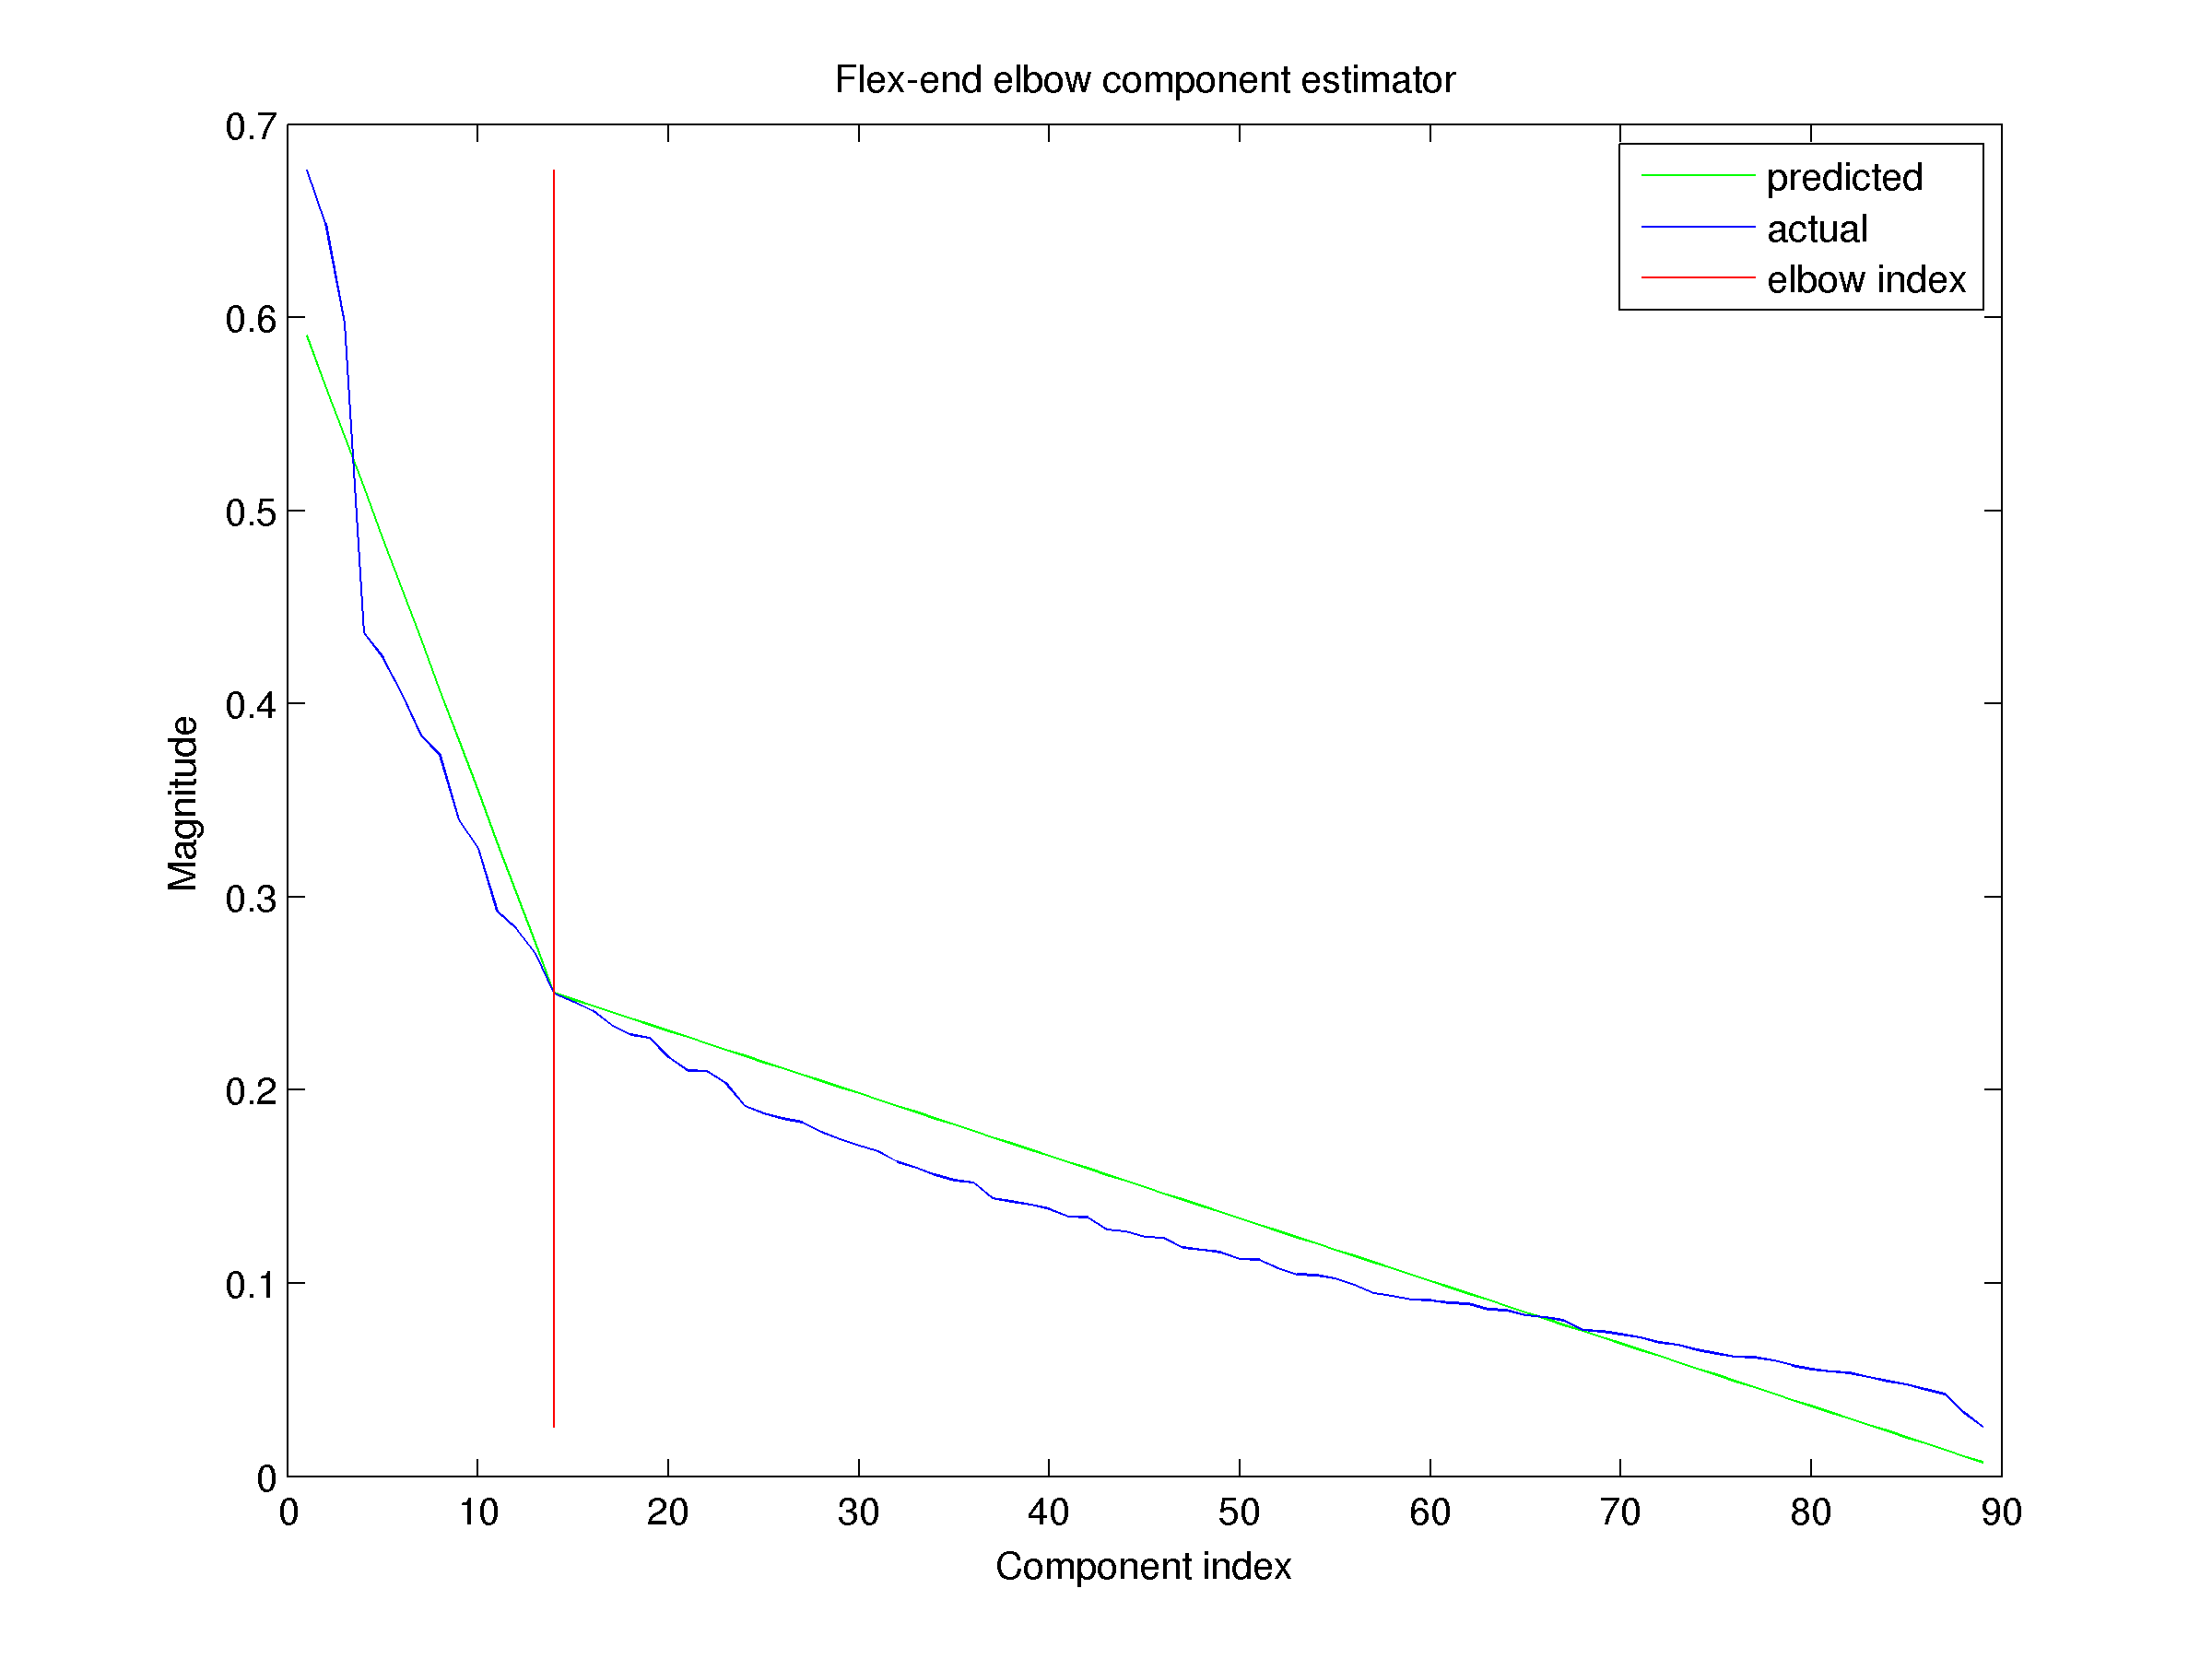
\includegraphics[width=0.9\linewidth]{100words-adj-800dim-lowercase-wmt-model-original-flex_end_elbow}
    \caption{Eigenvalues for each principal component of the 90 word vectors
    produced from the 101 word list.}
    \label{fig:101wordsunnormalizedpcaeigenvalues}
\end{figure}

\todo{switch the lambda plots in the results section to something properly labeled and scaled for easy comparison and without the elbow drawing}

\todo{make summary table plots into table rather than longtable environments so that they don't split across pages}

Table \ref{tab:101wordsRankingsUnnormalizedPCA} gives the highest and lowest
ranking words on the first 4 principal components of the unnormalized 90 word 
vectors. A more complete list can be found in Appendix 
\ref{app:rankedwordlists:101words:unnormalized}. The eigenvalues associated 
with each component are plotted in Figure 
\ref{fig:101wordsunnormalizedpcaeigenvalues}. The eigenvalue for a component is
proportional to the fraction of variance explained by that component.


\subsection{Normalized PCA}

\begin{longtable}[tbp]{| rllll |}
    \hline
      & \multicolumn{4}{c|}{\textbf{Component}} \\
    \textbf{Rank} & \textbf{1} & \textbf{2} & \textbf{3} & \textbf{4} \\
    \endhead
    \hline
    1 & irritable\_jj  & uncooperative\_jj  & negligent\_jj  & cold\_jj \\
    2 & uncooperative\_jj  & prompt\_jj  & uncooperative\_jj  & unreflective\_jj \\
    3 & self-pitying\_jj  & negligent\_jj  & imperturbable\_jj  & neat\_jj \\
    4 & extroverted\_jj  & systematic\_jj  & selfish\_jj  & self-pitying\_jj \\
    5 & unintelligent\_jj  & distrustful\_jj  & careless\_jj  & deep\_jj \\
    6 & talkative\_jj  & inconsistent\_jj  & prompt\_jj  & warm\_jj \\
    7 & rude\_jj  & insecure\_jj  & unreflective\_jj  & shallow\_jj \\
    \hline
    84 & steady\_jj  & uncharitable\_jj  & energetic\_jj  & thorough\_jj \\
    85 & simple\_jj  & talkative\_jj  & extroverted\_jj  & cooperative\_jj \\
    86 & systematic\_jj  & extroverted\_jj  & talkative\_jj  & talkative\_jj \\
    87 & innovative\_jj  & introspective\_jj  & pleasant\_jj  & kind\_jj \\
    88 & efficient\_jj  & energetic\_jj  & kind\_jj  & negligent\_jj \\
    89 & prompt\_jj  & considerate\_jj  & warm\_jj  & uncooperative\_jj \\
    90 & thorough\_jj  & imperturbable\_jj  & considerate\_jj  & considerate\_jj \\
    \hline
    \caption{The highest and lowest ranking words on the first 4 components 
    derived from normalized PCA of the 90 word vectors.}
    \label{tab:101wordsRankingsNormalizedPCA}
\end{longtable}


\begin{figure}[!tbp]
    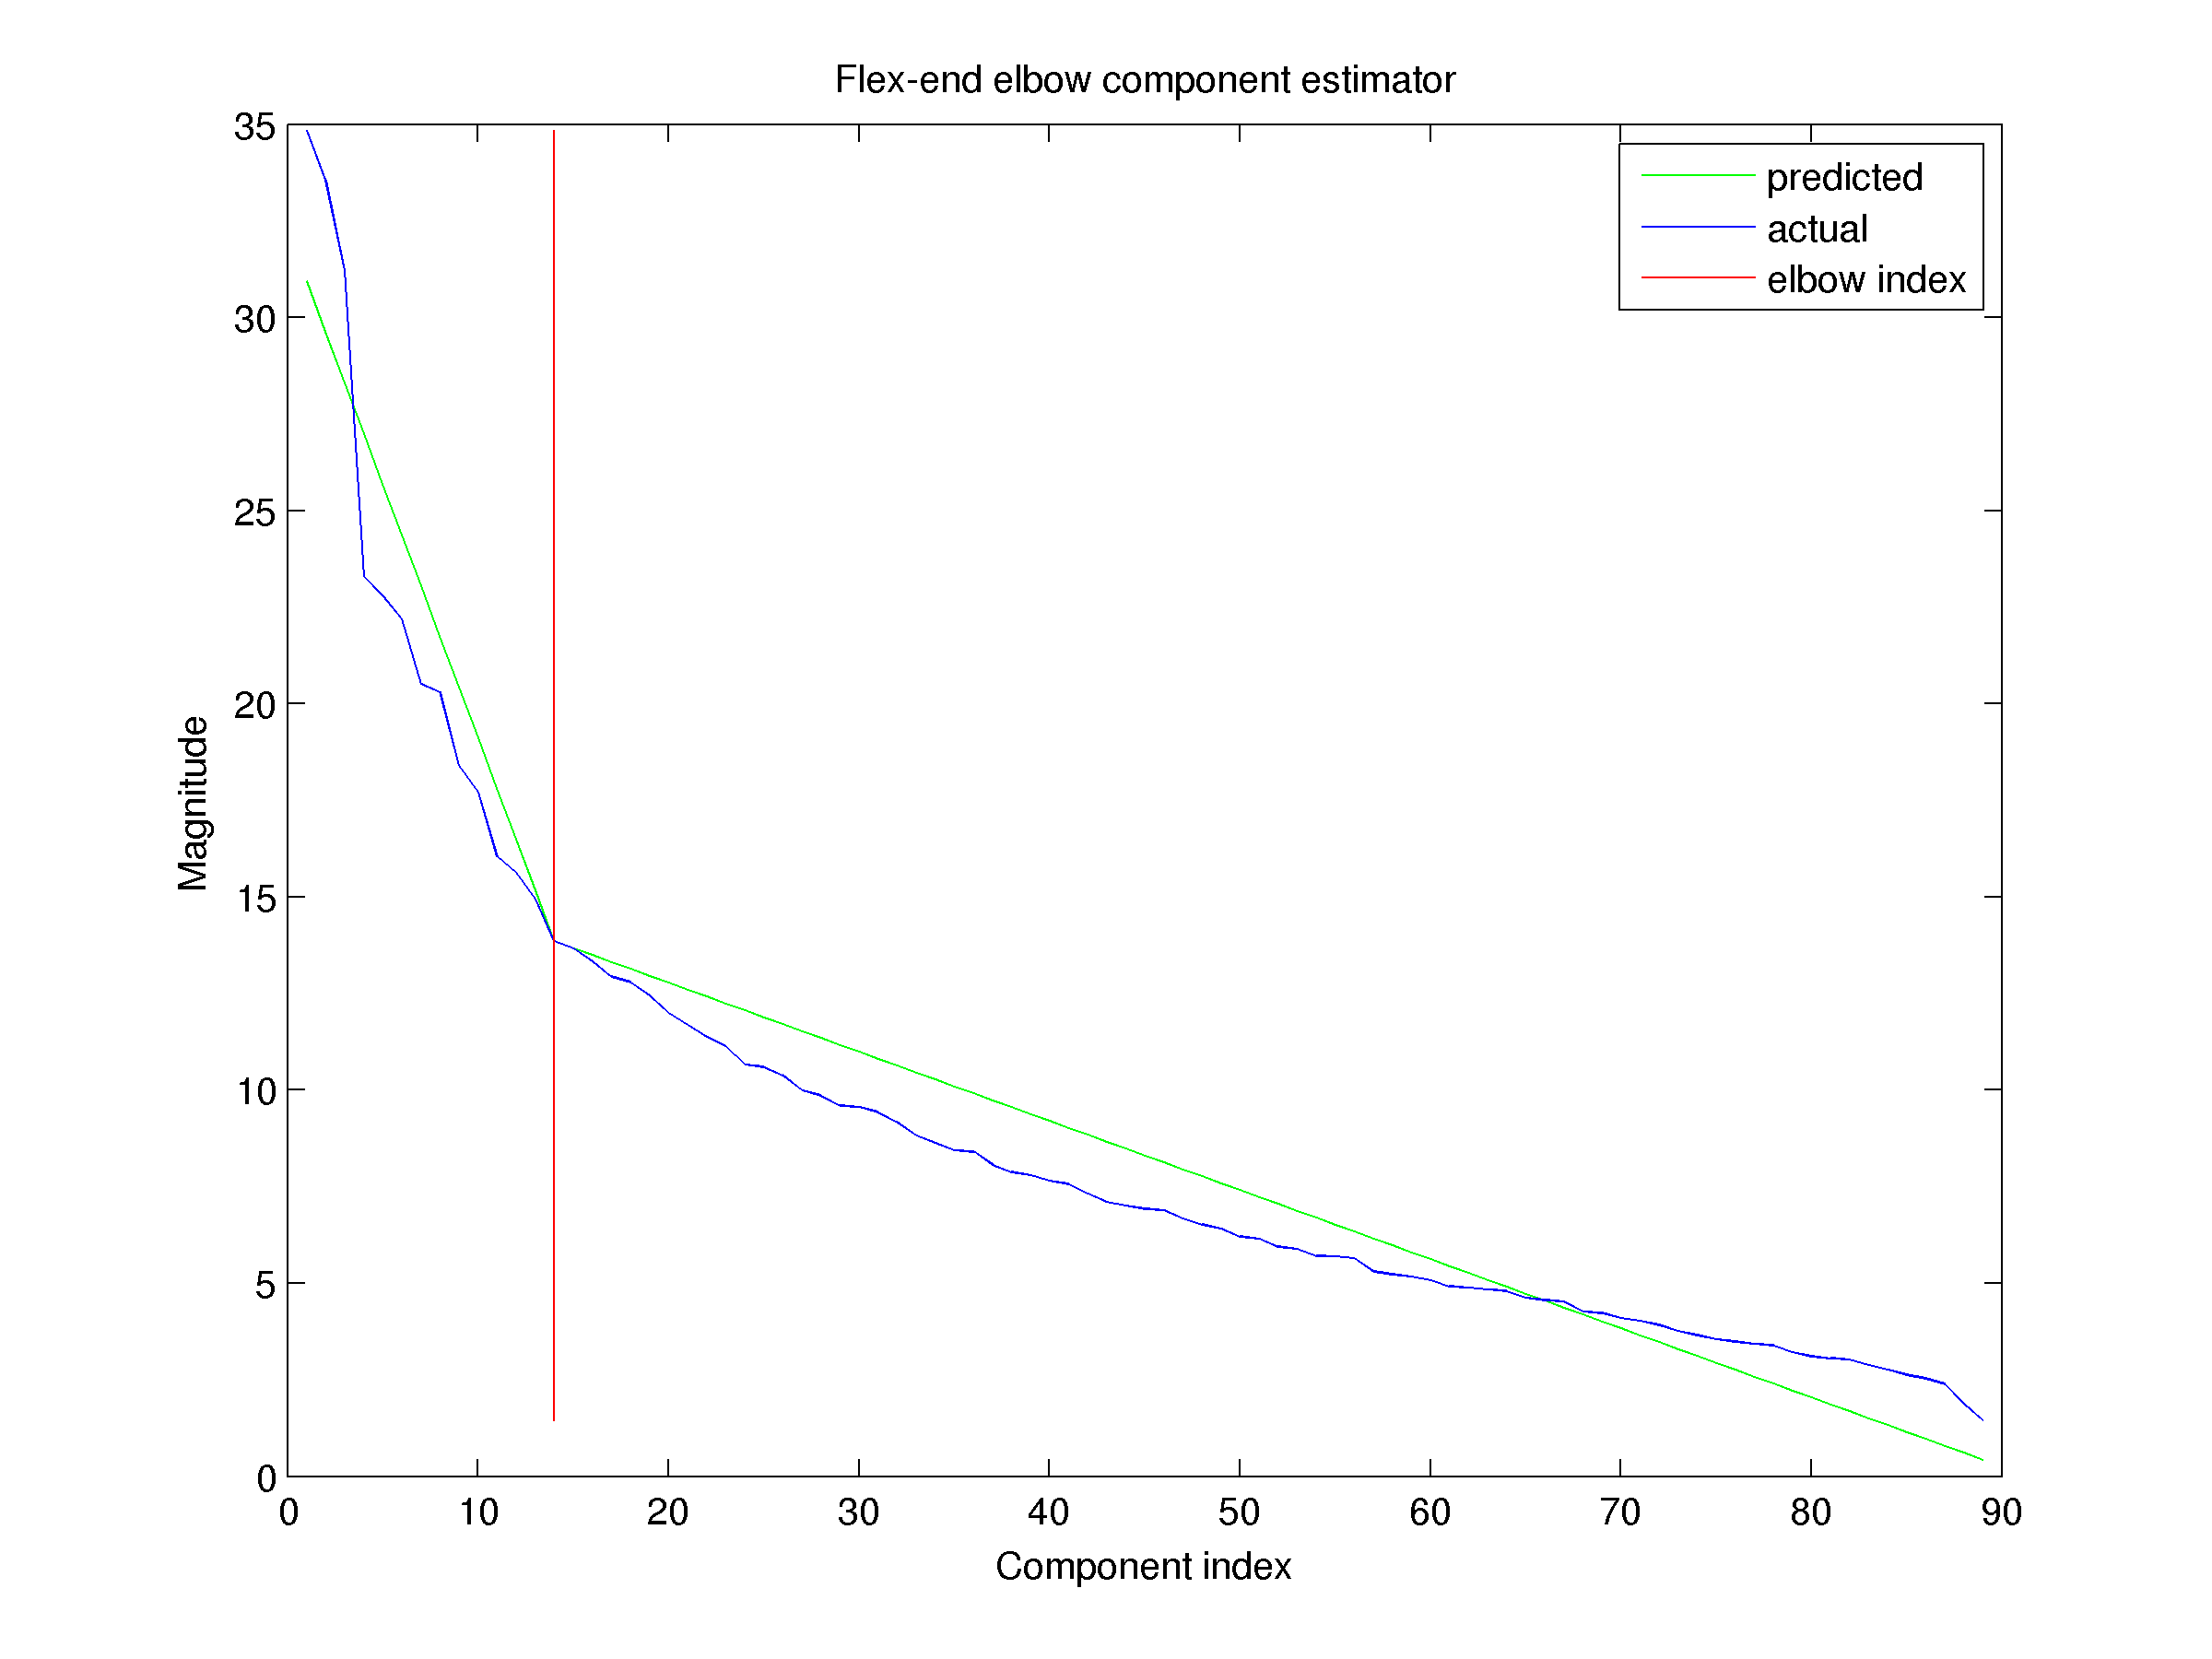
\includegraphics[width=0.9\linewidth]{100words-adj-800dim-lowercase-wmt-model-zscore-transformed-flex_end_elbow}
    \caption{Eigenvalues for each principal component of the 90 word vectors
    produced from the 101 word list after transforming to z-scores.}
    \label{fig:101wordsnormalizedpcaeigenvalues}
\end{figure}

Table \ref{tab:101wordsRankingsNormalizedPCA} gives the highest and lowest
ranking words on the first 4 principal components of the normalized 90 word 
vectors. A more complete list can be found in Appendix 
\ref{app:rankedwordlists:101words:normalized}. The eigenvalues associated 
with each component are plotted in Figure 
\ref{fig:101wordsnormalizedpcaeigenvalues}. The eigenvalue for a component is
proportional to the fraction of variance explained by that component.


\subsection{MDS}

\begin{longtable}[!htbp]{| rllll |}
    \hline
      & \multicolumn{4}{c|}{\textbf{Component}} \\
    \textbf{Rank} & \textbf{1} & \textbf{2} & \textbf{3} & \textbf{4} \\
    \endhead
    \hline
    1 & envious\_jj  & energetic\_jj  & imaginative\_jj  & active\_jj \\
    2 & jealous\_jj  & considerate\_jj  & artistic\_jj  & cooperative\_jj \\
    3 & self-pitying\_jj  & introspective\_jj  & innovative\_jj  & efficient\_jj \\
    4 & unkind\_jj  & pleasant\_jj  & unreflective\_jj  & sympathetic\_jj \\
    5 & bashful\_jj  & creative\_jj  & unadventurous\_jj  & assertive\_jj \\
    6 & fretful\_jj  & imaginative\_jj  & unimaginative\_jj  & unsympathetic\_jj \\
    7 & uncharitable\_jj  & extroverted\_jj  & creative\_jj  & distrustful\_jj \\
    \hline
    84 & systematic\_jj  & uncooperative\_jj  & careful\_jj  & bright\_jj \\
    85 & thorough\_jj  & inefficient\_jj  & quiet\_jj  & steady\_jj \\
    86 & efficient\_jj  & systematic\_jj  & warm\_jj  & shallow\_jj \\
    87 & complex\_jj  & sloppy\_jj  & cold\_jj  & warm\_jj \\
    88 & simple\_jj  & inconsistent\_jj  & fearful\_jj  & neat\_jj \\
    89 & practical\_jj  & unsystematic\_jj  & anxious\_jj  & deep\_jj \\
    90 & innovative\_jj  & negligent\_jj  & nervous\_jj  & cold\_jj \\
    \hline
    \caption{\todo{need to caption the table for 100words-adj-800dim-lowercase-wmt-model-mds-transformed-summary-table.tex} } \\
\end{longtable}


\begin{figure}[!tbp]
    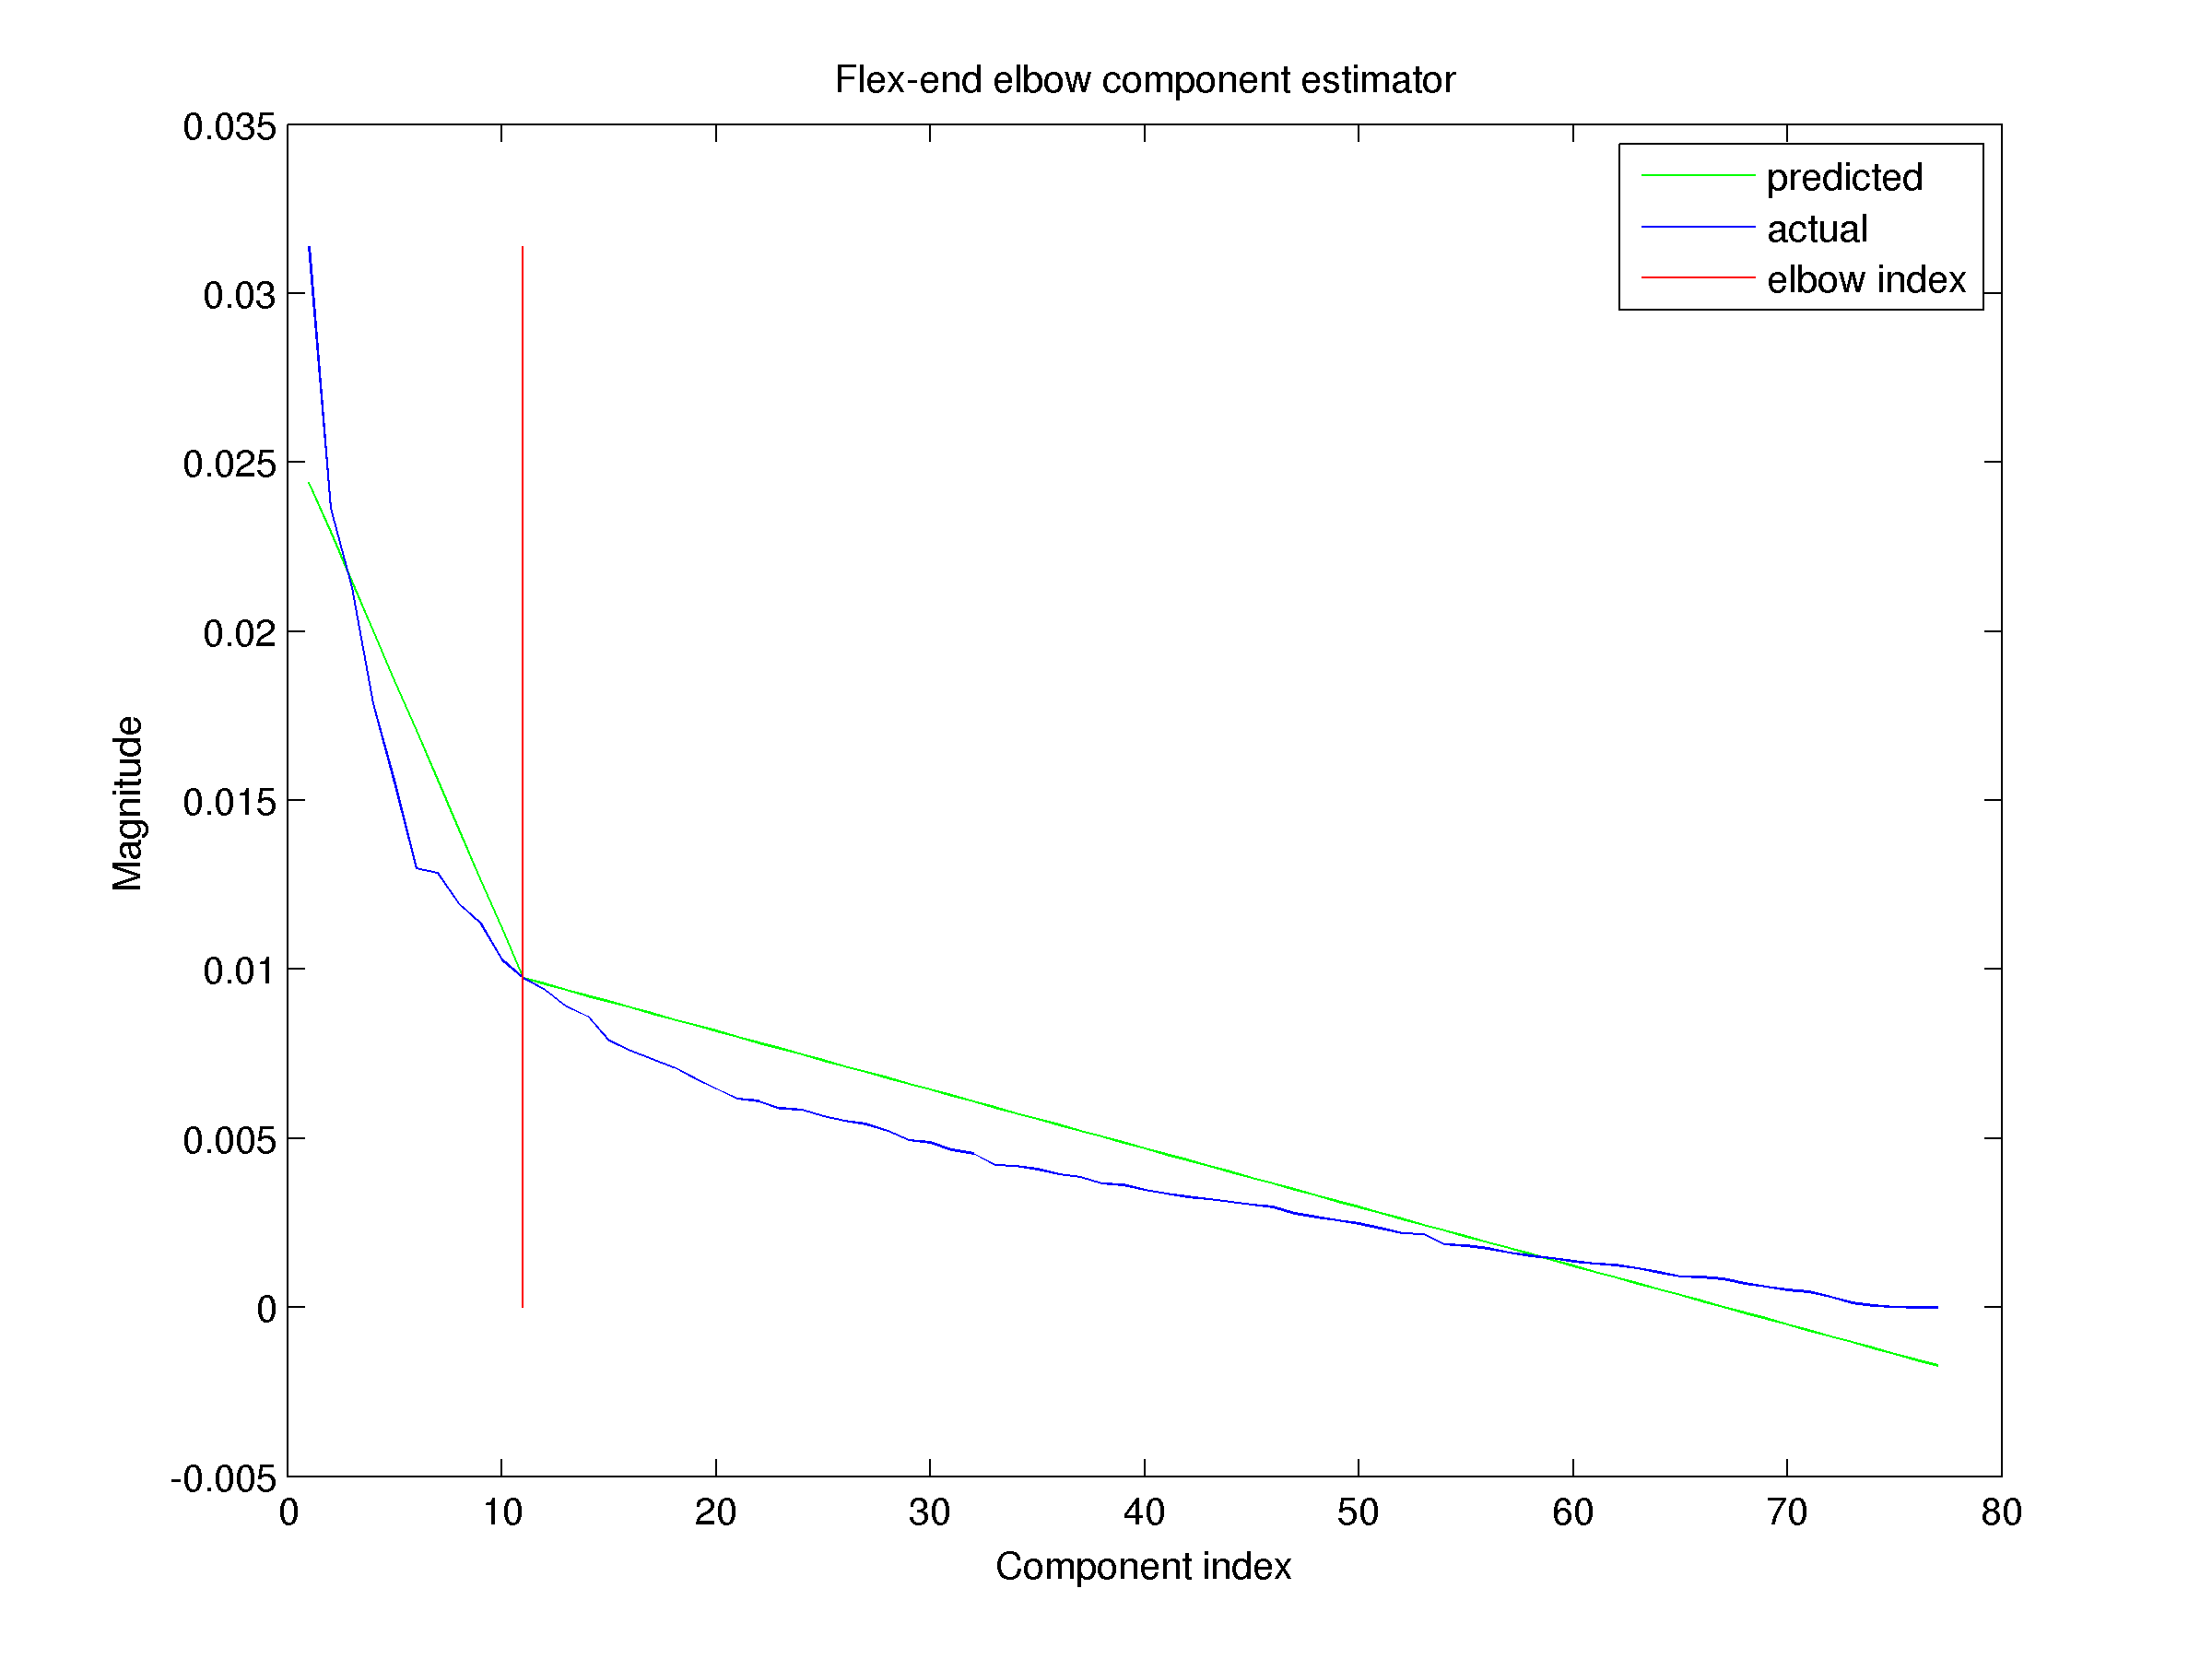
\includegraphics[width=0.9\linewidth]{100words-adj-800dim-lowercase-wmt-model-mds-transformed-flex_end_elbow}
    \caption{Eigenvalues for each principal component of the 90 word vectors
    produced from the 101 word list after multidimensional scaling.}
    \label{fig:101wordsmdseigenvalues}
\end{figure}

Table \ref{tab:101wordsRankingsMDS} gives the highest and lowest
ranking words on the first 4 principal components of the 90 word 
vectors after MDS. A more complete list can be found in Appendix 
\ref{app:rankedwordlists:101words:mds}. The eigenvalues associated 
with each component are plotted in Figure 
\ref{fig:101wordsmdseigenvalues}. The eigenvalue for a component is
proportional to the fraction of variance explained by that component.


\section{438 word set}

The 438 word set contained both adjectives and non-adjectives. Of these, 421 
were present in sufficient frequency to generate vectors within the memory 
constraints of the hardware on which we ran the skip-gram model. These words are 
listed in table \ref{tab:438wordsthatbecamevectors}. This produced 421 vectors 
on which further processing was performed. The adjectives carry the \_jj suffix 
from the Penn Treebank \todo{ref cite penn treebank} and the non-adjectives have 
no suffix.

\begin{longtable}[!htbp]{| llll |}
    \hline
    \endhead
   absent-minded\_jj & abusive\_jj & accommodating\_jj & active\_jj \\
   adaptable\_jj & adventurous\_jj & affectionate\_jj & agreeable\_jj \\
   aimless\_jj & aimlessness & aloofness & ambition \\
   ambitious\_jj & amiability & amiable\_jj & analytical\_jj \\
   animation & antagonistic\_jj & anxious\_jj & argumentative\_jj \\
   artistic\_jj & assertion & assertive\_jj & assured\_jj \\
   autonomous\_jj & bashful\_jj & belligerence & benevolent\_jj \\
   bigoted\_jj & bitter\_jj & boastful\_jj & bossiness \\
   bossy\_jj & brave\_jj & bright\_jj & bullheaded\_jj \\
   callousness & candor & carefree\_jj & careful\_jj \\
   careless\_jj & casual\_jj & caustic\_jj & caution \\
   cautious\_jj & charitable\_jj & cheerful\_jj & cold\_jj \\
   combative\_jj & communicative\_jj & compassionate\_jj & complex\_jj \\
   conceit & conceited\_jj & concise\_jj & condescending\_jj \\
   confident\_jj & considerate\_jj & consistent\_jj & contemplative\_jj \\
   conventional\_jj & conventionality & cooperation & cooperative\_jj \\
   cordial\_jj & cosmopolitan\_jj & courage & courageous\_jj \\
   courteous\_jj & courtesy & crabby\_jj & crafty\_jj \\
   cranky\_jj & creative\_jj & creativity & cruel\_jj \\
   cruelty & cultured\_jj & cunning & cunning\_jj \\
   curiosity & curious\_jj & curt\_jj & cynical\_jj \\
   daring & daring\_jj & deceit & deceitful\_jj \\
   decisive\_jj & decisiveness & deep\_jj & defensive\_jj \\
   deliberate\_jj & demanding\_jj & demonstrative\_jj & dependability \\
   dependable\_jj & depth & detached\_jj & devious\_jj \\
   dignified\_jj & dignity & diplomatic\_jj & direct\_jj \\
   dishonest\_jj & disorganization & disrespectful\_jj & distrust \\
   distrustful\_jj & docile\_jj & dominant\_jj & down-to-earth\_jj \\
   dull\_jj & earthiness & earthy\_jj & easygoing\_jj \\
   economical\_jj & efficiency & efficient\_jj & egocentric\_jj \\
   egotistical\_jj & emotional\_jj & emotionality & empathy \\
   energetic\_jj & enterprising\_jj & enthusiastic\_jj & envious\_jj \\
   envy & erratic\_jj & ethical\_jj & exacting\_jj \\
   excitable\_jj & exhibitionistic\_jj & explosive\_jj & expressive\_jj \\
   expressiveness & extravagant\_jj & extroverted\_jj & fastidious\_jj \\
   fear & fearful\_jj & firm\_jj & flamboyant\_jj \\
   flexibility & flexible\_jj & flippant\_jj & folksy\_jj \\
   foolhardy\_jj & forceful\_jj & foresighted\_jj & forgetful\_jj \\
   forgetfulness & formal\_jj & frank\_jj & fretful\_jj \\
   friendly\_jj & frivolity & frivolous\_jj & generosity \\
   generous\_jj & genial\_jj & greedy\_jj & gregarious\_jj \\
   gregariousness & gruff\_jj & grumpy\_jj & gullibility \\
   gullible\_jj & haphazard\_jj & happy-go-lucky\_jj & harsh\_jj \\
   helpful\_jj & homespun\_jj & honest\_jj & humble\_jj \\
   humor & humorous\_jj & ignorant\_jj & imaginative\_jj \\
   impersonal\_jj & impetuous\_jj & impolite\_jj & impractical\_jj \\
   impudent\_jj & inconsiderate\_jj & inconsistency & inconsistent\_jj \\
   indecisive\_jj & indecisiveness & independence & independent\_jj \\
   individualistic\_jj & industrious\_jj & inefficient\_jj & informal\_jj \\
   inhibition & innovative\_jj & inquisitive\_jj & insecure\_jj \\
   insecurity & insensitive\_jj & insight & insightful\_jj \\
   instability & intellectual\_jj & intellectuality & intelligence \\
   intelligent\_jj & introspective\_jj & intrusive\_jj & intrusiveness \\
   inventive\_jj & irritability & irritable\_jj & jealous\_jj \\
   jovial\_jj & joyless\_jj & kind\_jj & lazy\_jj \\
   leniency & lenient\_jj & lethargic\_jj & lethargy \\
   logic & logical\_jj & manipulative\_jj & mannerly\_jj \\
   meddlesome\_jj & meditative\_jj & melancholic\_jj & merry\_jj \\
   meticulous\_jj & mischievous\_jj & miserly\_jj & modest\_jj \\
   modesty & moody\_jj & moral\_jj & morality \\
   morose\_jj & natural\_jj & naturalness & naïve\_jj \\
   negligence & negligent\_jj & nervous\_jj & nonconforming\_jj \\
   nonconformity & nosey\_jj & obliging\_jj & obstinate\_jj \\
   opportunistic\_jj & optimism & optimistic\_jj & orderly\_jj \\
   organization & organized\_jj & passionless\_jj & passive\_jj \\
   passivity & patient\_jj & peaceful\_jj & perceptive\_jj \\
   persistence & persistent\_jj & pessimism & pessimistic\_jj \\
   philosophical\_jj & placidity & playful\_jj & playfulness \\
   pleasant\_jj & polite\_jj & pomposity & pompous\_jj \\
   precise\_jj & precision & predictability & predictable\_jj \\
   prejudice & prejudiced\_jj & principled\_jj & prompt\_jj \\
   proud\_jj & punctual\_jj & punctuality & purposeful\_jj \\
   quarrelsome\_jj & quiet & quiet\_jj & rambunctious\_jj \\
   rash\_jj & reasonable\_jj & rebellious\_jj & reckless\_jj \\
   recklessness & refined\_jj & reliable\_jj & reserve \\
   reserved\_jj & respectful\_jj & responsible\_jj & restrained\_jj \\
   rude\_jj & rudeness & ruthless\_jj & scatterbrained\_jj \\
   scornful\_jj & secretive\_jj & self-critical\_jj & self-disciplined\_jj \\
   self-esteem & self-indulgent\_jj & self-pitying\_jj & selfish\_jj \\
   selfishness & selfless\_jj & sentimental\_jj & shallow\_jj \\
   shallowness & shy\_jj & shyness & silence \\
   silent\_jj & simple\_jj & sincere\_jj & skeptical\_jj \\
   sloppy\_jj & sloth & slothful\_jj & sluggish\_jj \\
   sly\_jj & smart\_jj & smug\_jj & snobbish\_jj \\
   sociable\_jj & somber\_jj & sophisticated\_jj & sophistication \\
   spirit & spirited\_jj & spontaneity & spontaneous\_jj \\
   steady\_jj & stinginess & stingy\_jj & straightforward\_jj \\
   stubborn\_jj & stubbornness & stupidity & submissive\_jj \\
   suggestible\_jj & surliness & surly\_jj & suspicious\_jj \\
   sympathetic\_jj & systematic\_jj & tactful\_jj & tactless\_jj \\
   talkative\_jj & talkativeness & temperamental\_jj & tempestuous\_jj \\
   tenacious\_jj & thorough\_jj & thoughtless\_jj & thoughtlessness \\
   thrift & thrifty\_jj & timid\_jj & touchy\_jj \\
   traditional\_jj & trustful\_jj & truthful\_jj & unadventurous\_jj \\
   unaggressive\_jj & unambitious\_jj & unassuming\_jj & unconventional\_jj \\
   uncritical\_jj & undemanding\_jj & undependable\_jj & underhanded\_jj \\
   understanding & understanding\_jj & unemotional\_jj & unexcitable\_jj \\
   unfriendliness & unfriendly\_jj & ungracious\_jj & unimaginative\_jj \\
   uninhibited\_jj & unintelligent\_jj & unkind\_jj & unobservant\_jj \\
   unpredictable\_jj & unreflective\_jj & unreliable\_jj & unrestrained\_jj \\
   unscrupulous\_jj & unsociable\_jj & unstable\_jj & unsympathetic\_jj \\
   unsystematic\_jj & vain\_jj & verbal\_jj & verbose\_jj \\
   vigorous\_jj & vindictive\_jj & vivacious\_jj & volatile\_jj \\
   volatility & warm\_jj & warmth & wishy-washy\_jj \\
   withdrawn\_jj & witty\_jj & wordy\_jj & worldly\_jj \\
   zestful\_jj & & &\\
    \hline
    \caption{The 421 words from the list of 438 for which vectors were generated.}
    \label{tab:438wordsthatbecamevectors}
\end{longtable}



\subsection{Unnormalized PCA}

\begin{longtable}[!htbp]{| rllll |}
    \hline
      & \multicolumn{4}{c|}{\textbf{Component}} \\
    \textbf{Rank} & \textbf{1} & \textbf{2} & \textbf{3} & \textbf{4} \\
    \endhead
    \hline
    1 & sociable\_jj  & callousness  & abusive\_jj  & sincere\_jj \\
    2 & vivacious\_jj  & selfishness  & inconsiderate\_jj  & considerate\_jj \\
    3 & considerate\_jj  & gullibility  & selfish\_jj  & dignity \\
    4 & easygoing\_jj  & stupidity  & disrespectful\_jj  & courage \\
    5 & witty\_jj  & recklessness  & insensitive\_jj  & selfless\_jj \\
    6 & affectionate\_jj  & rudeness  & ignorant\_jj  & honest\_jj \\
    7 & talkative\_jj  & deceit  & dishonest\_jj  & courageous\_jj \\
    \hline
    415 & caution  & optimistic\_jj  & warmth  & fretful\_jj \\
    416 & sluggish\_jj  & easygoing\_jj  & sophistication  & sluggish\_jj \\
    417 & intelligence  & efficient\_jj  & naturalness  & lethargic\_jj \\
    418 & cooperation  & reliable\_jj  & earthiness  & lethargy \\
    419 & volatility  & friendly\_jj  & expressiveness  & irritability \\
    420 & instability  & considerate\_jj  & spontaneity  & irritable\_jj \\
    421 & negligence  & sociable\_jj  & playfulness  & absent-minded\_jj \\
    \hline
    \caption{\todo{need to caption the table for 439words-adj-800dim-lowercase-wmt-model-original-summary-table.tex} } \\
\end{longtable}


\begin{figure}[!tbp]
    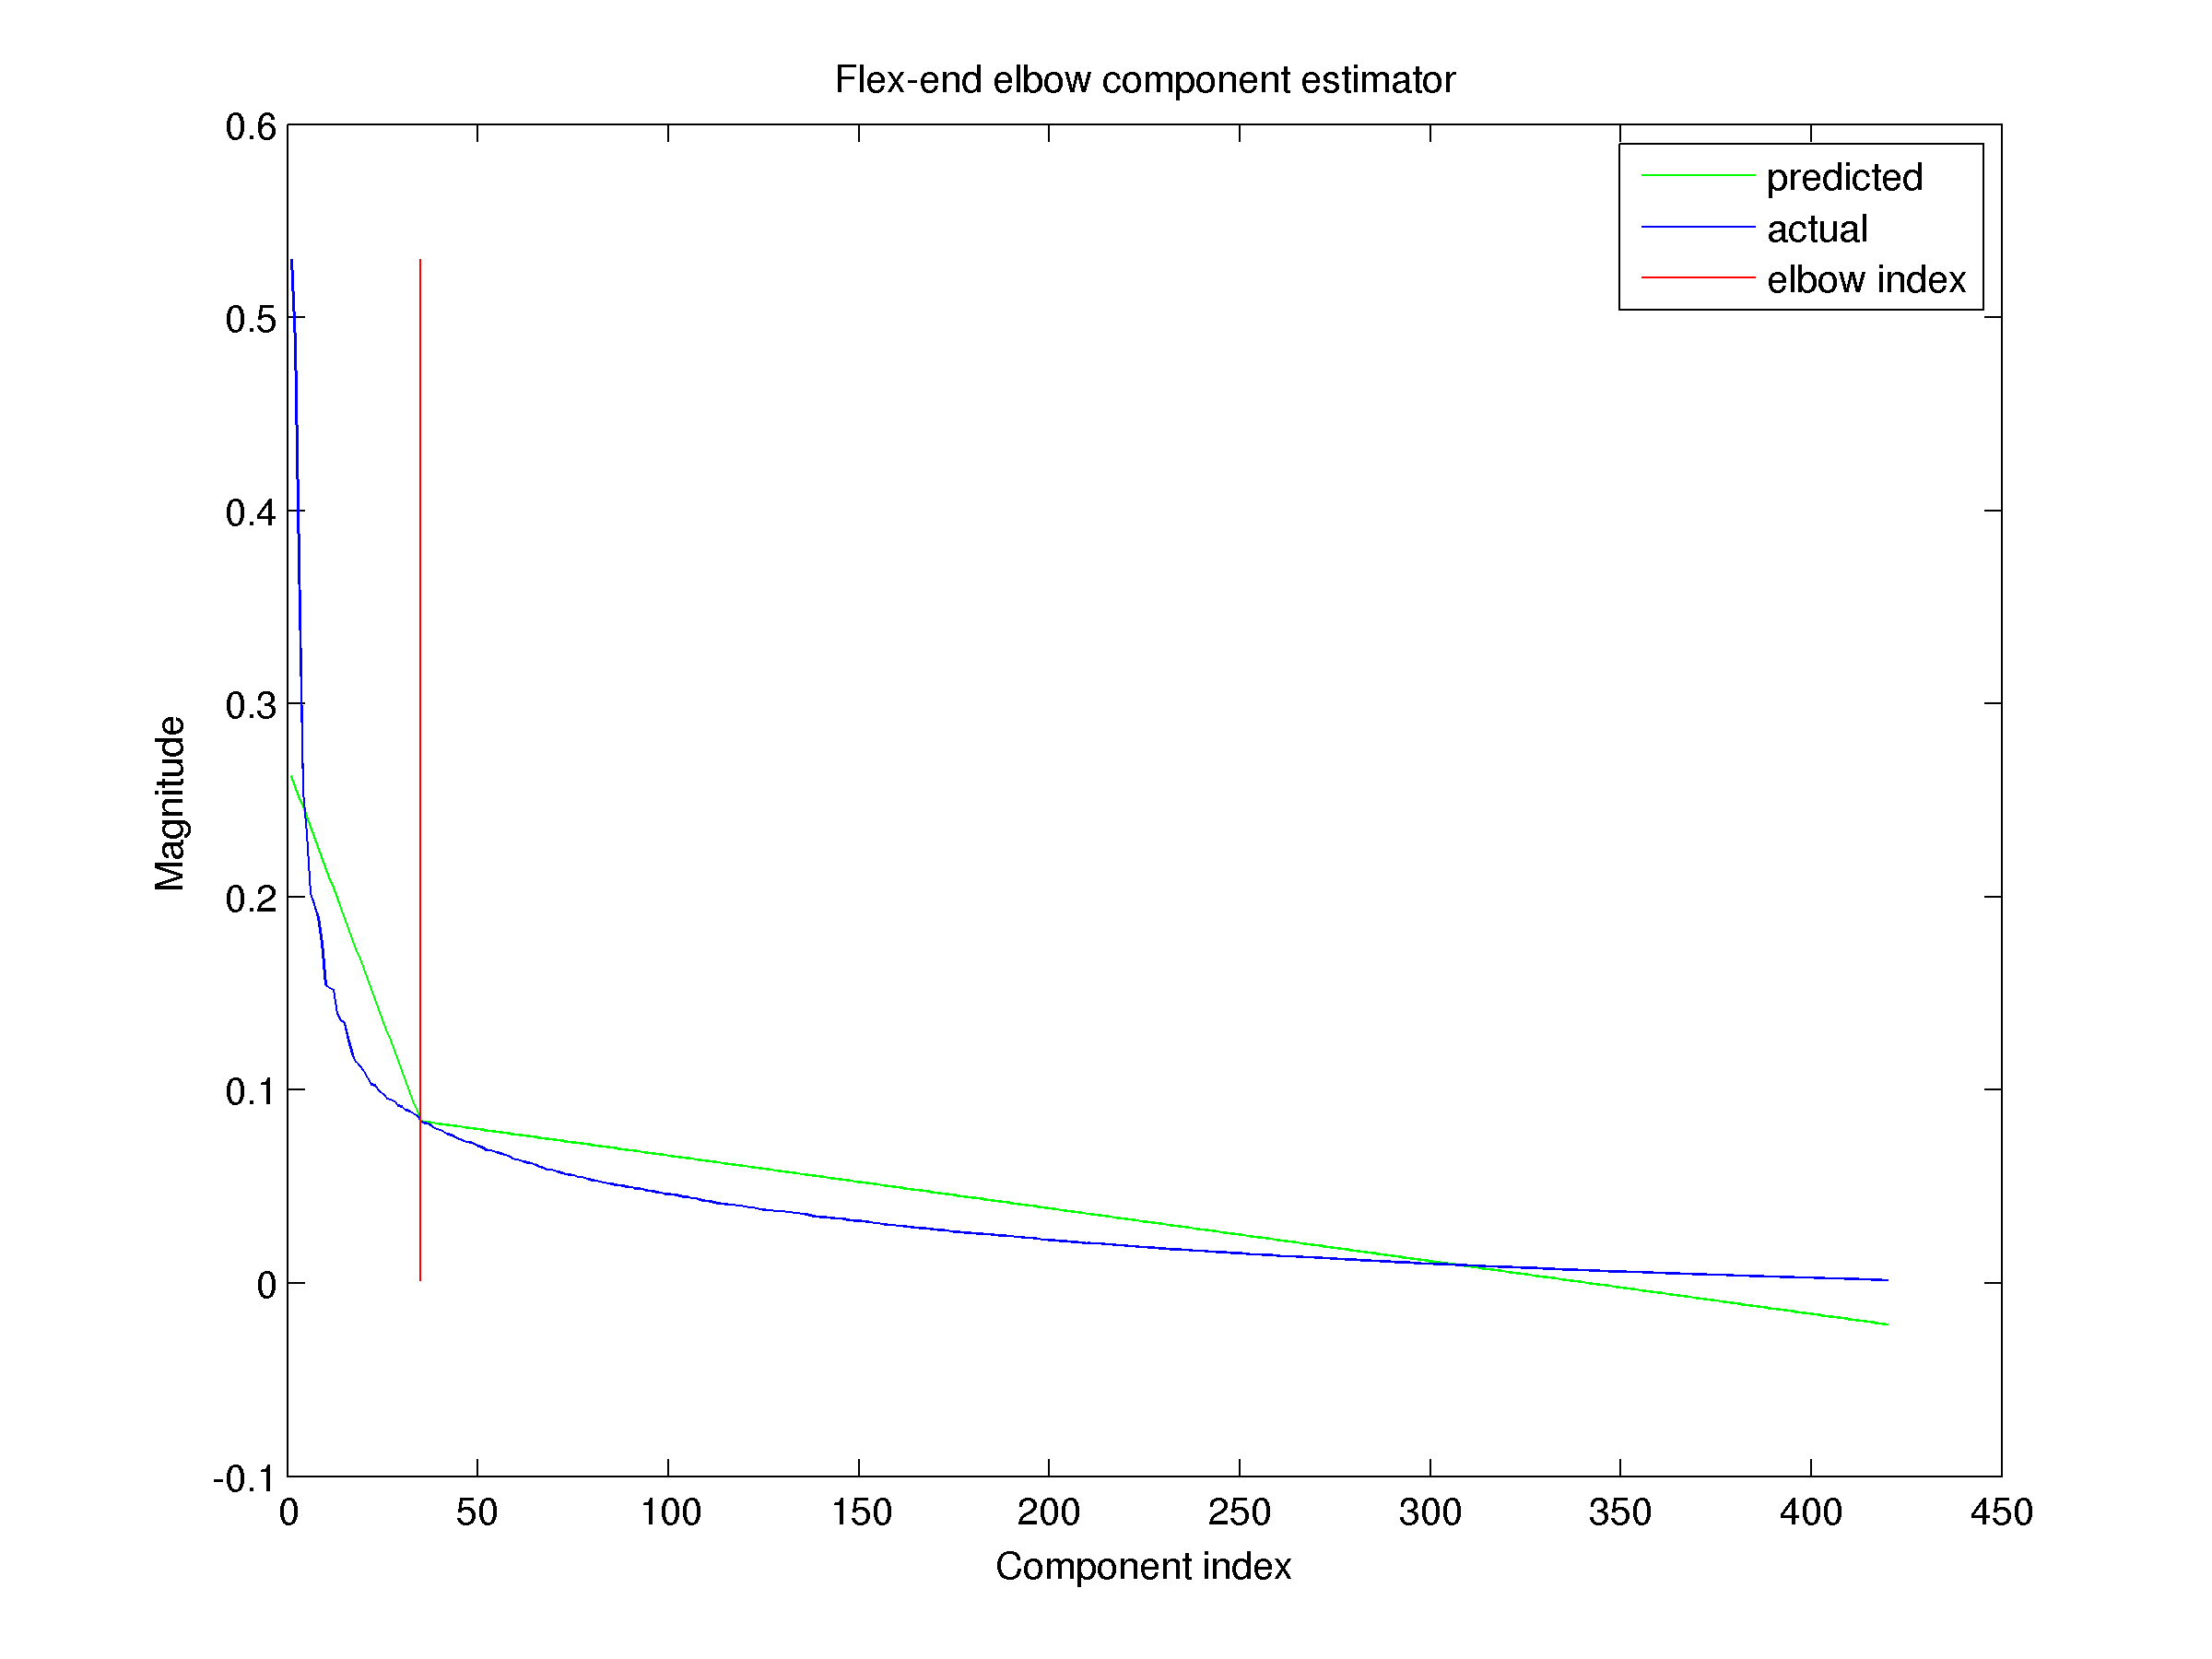
\includegraphics[width=0.9\linewidth]{439words-adj-800dim-lowercase-wmt-model-original-flex_end_elbow}
    \caption{Eigenvalues for each principal component of the 421 word vectors
    produced from the 438 word list.}
    \label{fig:438wordsunnormalizedpcaeigenvalues}
\end{figure}

Table \ref{tab:438wordsRankingsUnnormalizedPCA} gives the highest and lowest
ranking words on the first 4 principal components of the unnormalized 421 word 
vectors. A more complete list can be found in Appendix 
\ref{app:rankedwordlists:438words:unnormalized}.


\subsection{Normalized PCA}

\begin{longtable}[!htbp]{| rllll |}
    \hline
      & \multicolumn{4}{c|}{\textbf{Component}} \\
    \textbf{Rank} & \textbf{1} & \textbf{2} & \textbf{3} & \textbf{4} \\
    \endhead
    \hline
    1 & sociable\_jj  & callousness  & abusive\_jj  & sincere\_jj \\
    2 & vivacious\_jj  & selfishness  & inconsiderate\_jj  & considerate\_jj \\
    3 & considerate\_jj  & gullibility  & insensitive\_jj  & dignity \\
    4 & easygoing\_jj  & recklessness  & selfish\_jj  & courage \\
    5 & witty\_jj  & stupidity  & ignorant\_jj  & selfless\_jj \\
    6 & talkative\_jj  & rudeness  & disrespectful\_jj  & courageous\_jj \\
    7 & affectionate\_jj  & deceit  & dishonest\_jj  & honest\_jj \\
    \hline
    415 & caution  & dependable\_jj  & warmth  & erratic\_jj \\
    416 & sluggish\_jj  & easygoing\_jj  & earthiness  & lethargic\_jj \\
    417 & intelligence  & efficient\_jj  & sophistication  & sluggish\_jj \\
    418 & cooperation  & reliable\_jj  & naturalness  & lethargy \\
    419 & volatility  & friendly\_jj  & expressiveness  & irritability \\
    420 & instability  & considerate\_jj  & spontaneity  & irritable\_jj \\
    421 & negligence  & sociable\_jj  & playfulness  & absent-minded\_jj \\
    \hline
    \caption{\todo{need to caption the table for 439words-adj-800dim-lowercase-wmt-model-zscore-transformed-summary-table.tex} } \\
\end{longtable}


\begin{figure}[!tbp]
    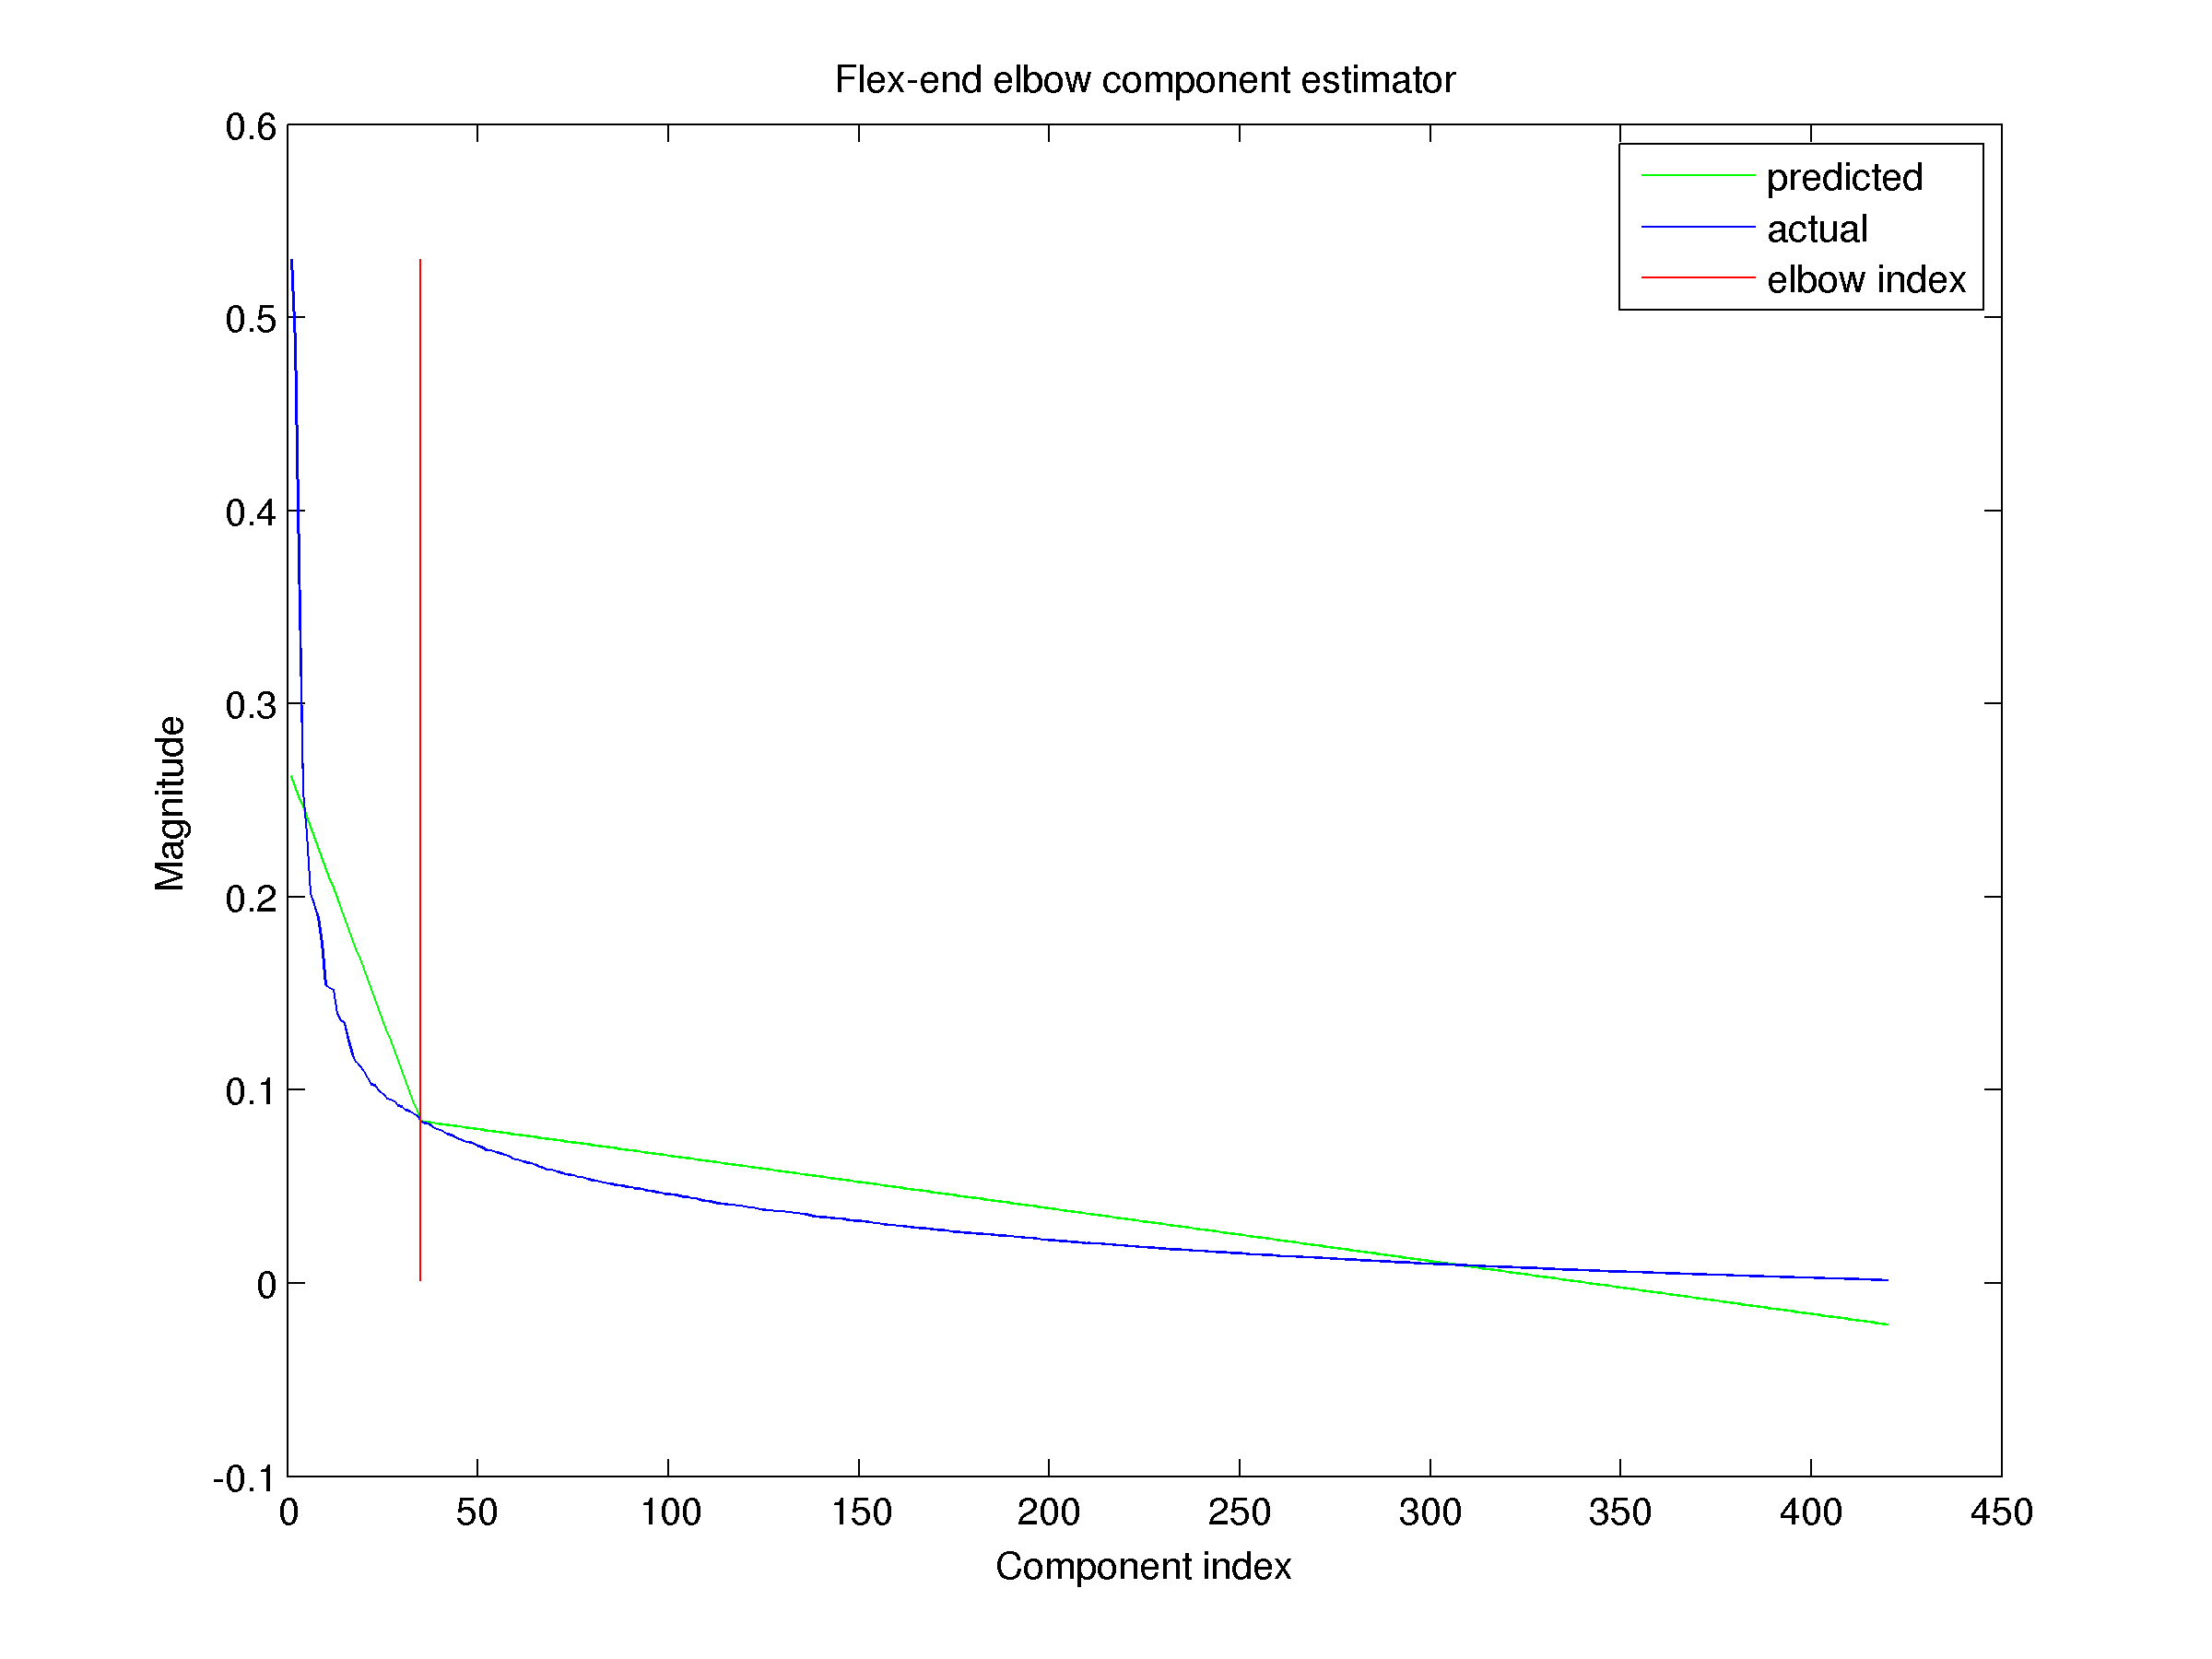
\includegraphics[width=0.9\linewidth]{439words-adj-800dim-lowercase-wmt-model-original-flex_end_elbow}
    \caption{Eigenvalues for each principal component of the 421 z-score 
    normalized word vectors produced from the 438 word list.}
    \label{fig:438wordsnormalizedpcaeigenvalues}
\end{figure}

Table \ref{tab:438wordsRankingsNormalizedPCA} gives the highest and lowest
ranking words on the first 4 principal components of the z-score normalized 421 
word vectors. A more complete list can be found in Appendix 
\ref{app:rankedwordlists:438words:normalized}.

\subsection{MDS}

\begin{longtable}[!htbp]{| rllll |}
    \hline
      & \multicolumn{4}{c|}{\textbf{Component}} \\
    \textbf{Rank} & \textbf{1} & \textbf{2} & \textbf{3} & \textbf{4} \\
    \endhead
    \hline
    1 & self-pitying\_jj  & sociable\_jj  & ignorant\_jj  & innovative\_jj \\
    2 & scatterbrained\_jj  & cheerful\_jj  & dishonest\_jj  & dishonest\_jj \\
    3 & pomposity  & vivacious\_jj  & insensitive\_jj  & intelligent\_jj \\
    4 & mischievous\_jj  & easygoing\_jj  & greedy\_jj  & ethical\_jj \\
    5 & sly\_jj  & considerate\_jj  & disrespectful\_jj  & imaginative\_jj \\
    6 & pompous\_jj  & enthusiastic\_jj  & bigoted\_jj  & truthful\_jj \\
    7 & snobbish\_jj  & dependable\_jj  & unfriendly\_jj  & honest\_jj \\
    \hline
    415 & volatile\_jj  & passivity  & spirit  & lethargy \\
    416 & reasonable\_jj  & deceit  & persistence  & irritable\_jj \\
    417 & flexibility  & recklessness  & playfulness  & cold\_jj \\
    418 & reliable\_jj  & gullibility  & spontaneity  & anxious\_jj \\
    419 & direct\_jj  & selfishness  & precision  & lethargic\_jj \\
    420 & cooperation  & callousness  & warmth  & sluggish\_jj \\
    421 & consistent\_jj  & stupidity  & creativity  & nervous\_jj \\
    \hline
    \caption{The highest and lowest ranking words on the first 4 components 
    derived from performaing MDS on the 421 word vectors.}
    \label{tab:438wordsRankingsMDS}
\end{longtable}


Table \ref{tab:438wordsRankingsMDS} gives the highest and lowest
ranking words on the first 4 principal components of the 421 word 
vectors after MDS. A more complete list can be found in Appendix 
\ref{app:rankedwordlists:438words:mds}.

\begin{figure}[!tbp]
    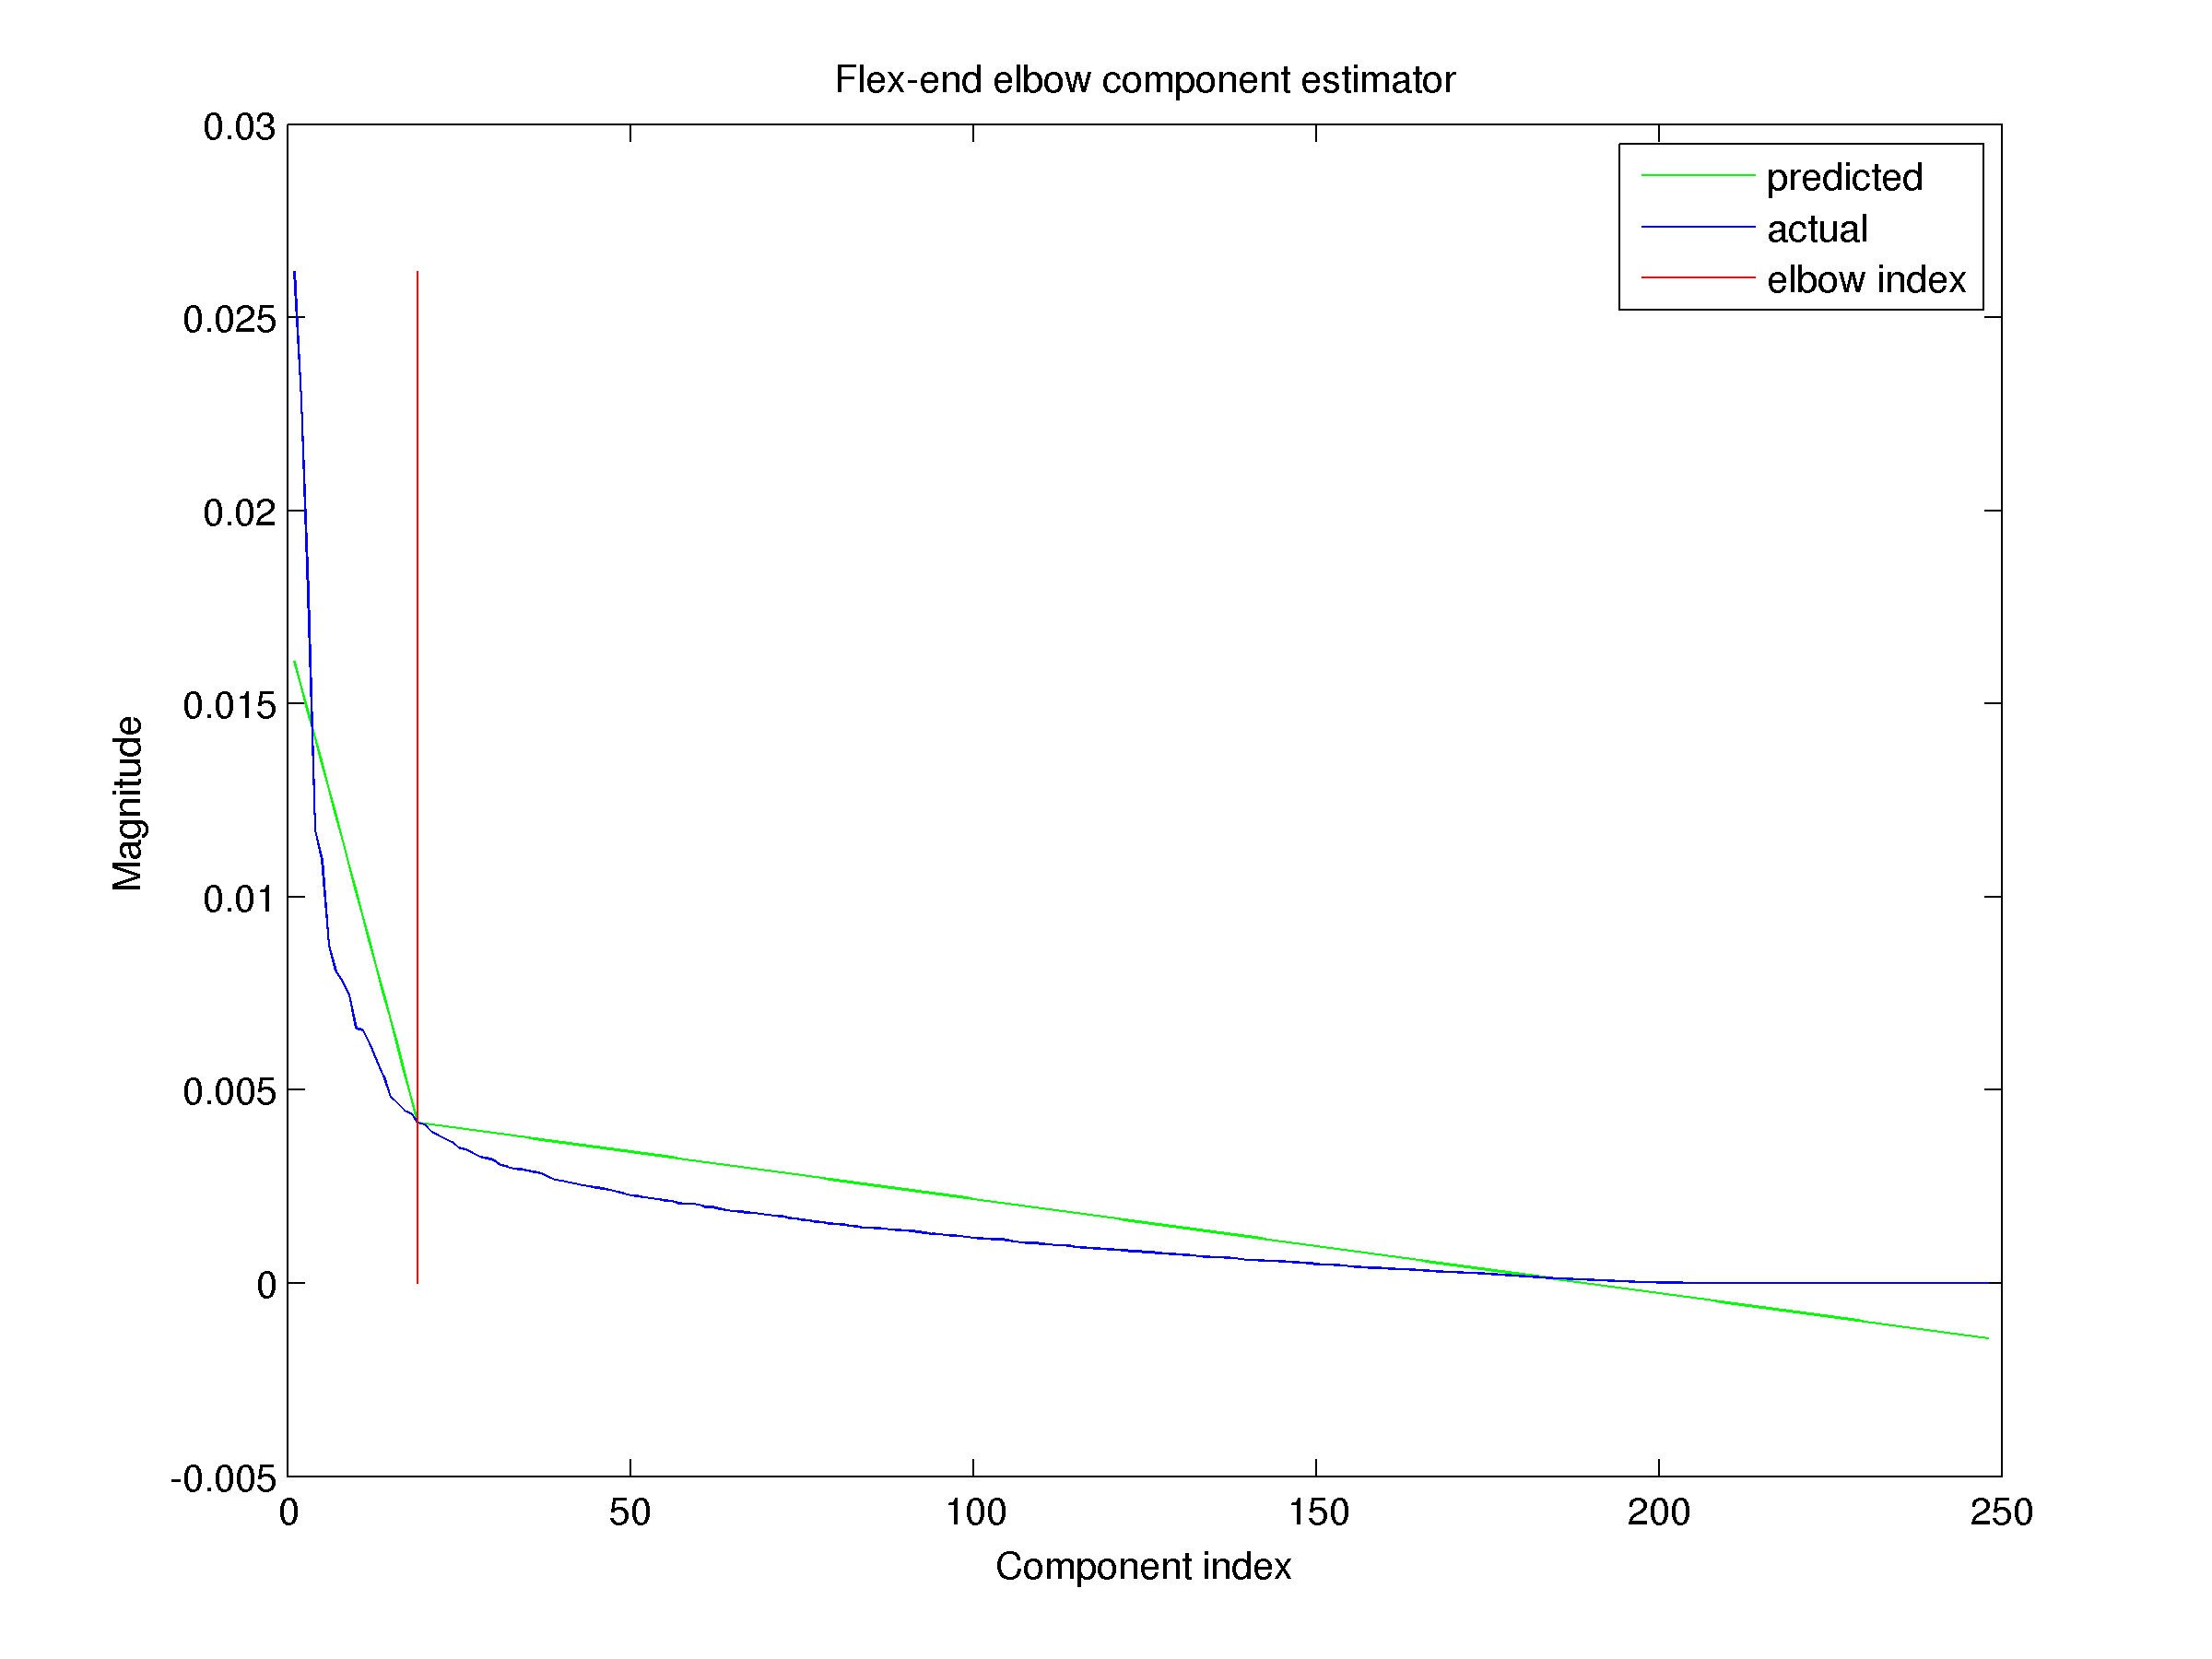
\includegraphics[width=0.9\linewidth]{439words-adj-800dim-lowercase-wmt-model-mds-transformed-flex_end_elbow}
    \caption{Eigenvalues for each principal component of the 421 word vectors
    produced from the 438 word list after multidimensional scaling.}
    \label{fig:438wordsmdseigenvalues}
\end{figure}


\section{101 and 438 word sets combined}

There were a few words in the 101 word list that were not also in the 438 word list. So, for completeness, we also ran the same analysis with the two lists combined. In the combined list, 430 words were frequent enough to be assigned vectors given our memory constraints. To save space, we only list the 9 words not used in the 438 word list analysis in Table \ref{tab:additionalwordsincombined}.

\begin{table}[!htbp]
    \begin{tabular}{| llll |}
        \hline
        bold\_jj & conscientious\_jj & high-strung\_jj & imperturbable\_jj \\
        neat\_jj & practical\_jj & uncharitable\_jj & uncooperative\_jj \\
        unsophisticated\_jj & & &\\
        \hline
    \end{tabular}
    \caption{The 9 words present in the 90 word vectors from the 101 word 
    analysis that were not present in the 421 word vector list in the 438 
    word analysis}
    \label{tab:additionalwordsincombined}
\end{table}

As can be seen from \ref{fig:439vs439and100} the most significant components
of the combined word-list are almost identical to those of the 439 word-list
alone. Thus, we do not show them here. See the appendices for details.

\begin{figure}[!tbp]
    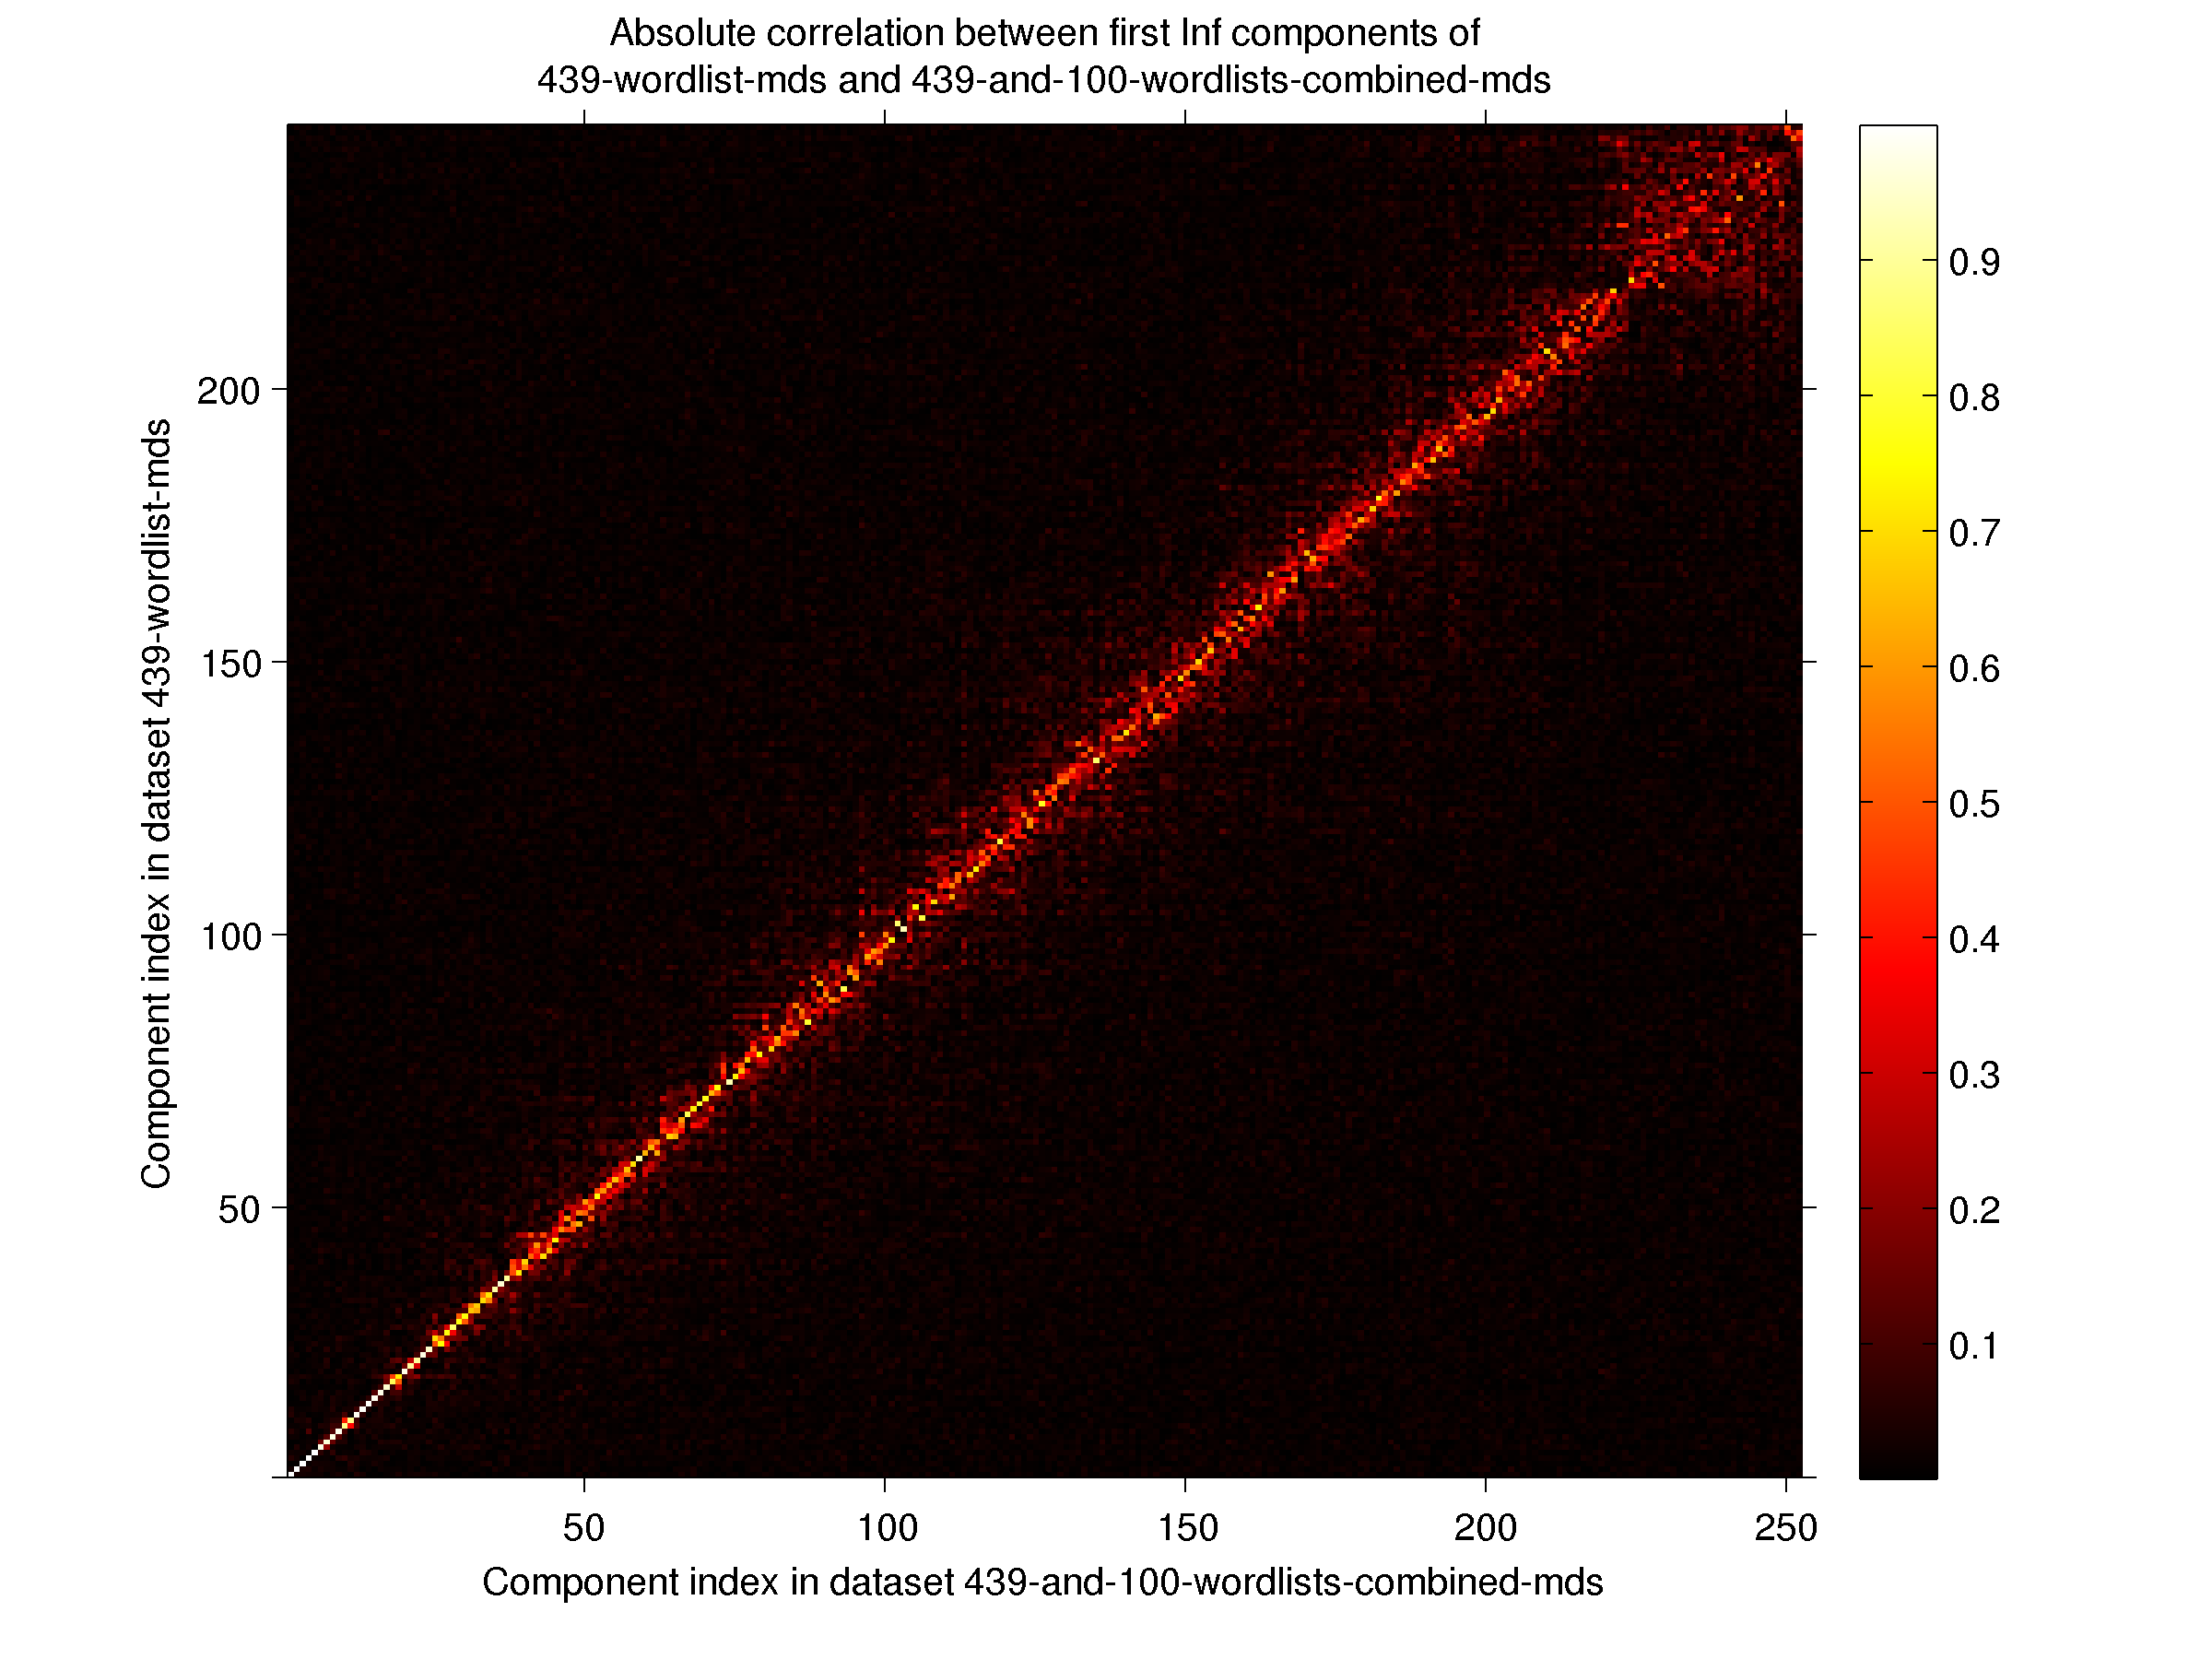
\includegraphics[width=0.9\linewidth]{439-vs-439and100-from-800dim-lowercase-wmt-model-correlations}
    \caption{Correlations between the first 52 MDS vectors generated from the 
    439 word list alone and first 52 the vectors generated from the combined
    439 word and 101 word lists.}
    \label{fig:439vs439and100}
\end{figure}

\section{2797 word set}

The 2797 word list contained adjectives and nouns. The nouns were not merely
qualities but also categories of people. With the spelling corrections and 
variants, there were 2810 words before tagging. After tagging, there were
1860 vectors generated from this list.

\subsection{Unnormalized PCA}

\begin{longtable}[!htbp]{| rllll |}
    \hline
      & \multicolumn{4}{c|}{\textbf{Component}} \\
    \textbf{Rank} & \textbf{1} & \textbf{2} & \textbf{3} & \textbf{4} \\
    \endhead
    \hline
    1 & stringent\_jj  & warm\_jj  & considerate\_jj  & loyal\_jj \\
    2 & beneficial\_jj  & elegant\_jj  & sociable\_jj  & objector \\
    3 & indirect\_jj  & vibrant\_jj  & courteous\_jj  & staunch\_jj \\
    4 & contentious\_jj  & savant  & trustworthy\_jj  & devout\_jj \\
    5 & prudent\_jj  & sparkling\_jj  & articulate\_jj  & sociable\_jj \\
    6 & dependent\_jj  & luxurious\_jj  & open-minded\_jj  & alcoholic \\
    7 & lax\_jj  & graceful\_jj  & approachable\_jj  & avid\_jj \\
    \hline
    1854 & sardonic\_jj  & slanderous\_jj  & broiler  & contrived\_jj \\
    1855 & guileless\_jj  & selfish\_jj  & soft-shelled\_jj  & didactic\_jj \\
    1856 & go-getter  & cowardly\_jj  & bendable\_jj  & defamatory\_jj \\
    1857 & self-possessed\_jj  & deceitful\_jj  & pixy  & imprecise\_jj \\
    1858 & girlish\_jj  & untruthful\_jj  & butterfly  & dissonant\_jj \\
    1859 & vivacious\_jj  & bigoted\_jj  & gingery\_jj  & limpid\_jj \\
    1860 & mousy\_jj  & defamatory\_jj  & comforter  & unvarying\_jj \\
    \hline
    \caption{The highest and lowest ranking words on the first 4 components 
    derived from unnormalized PCA of the 1860 word vectors 
    derived from the 2797 word list.} 
    \label{tab:2797wordsRankingsUnnormalizedPCA}
\end{longtable}


\begin{figure}[!tbp]
    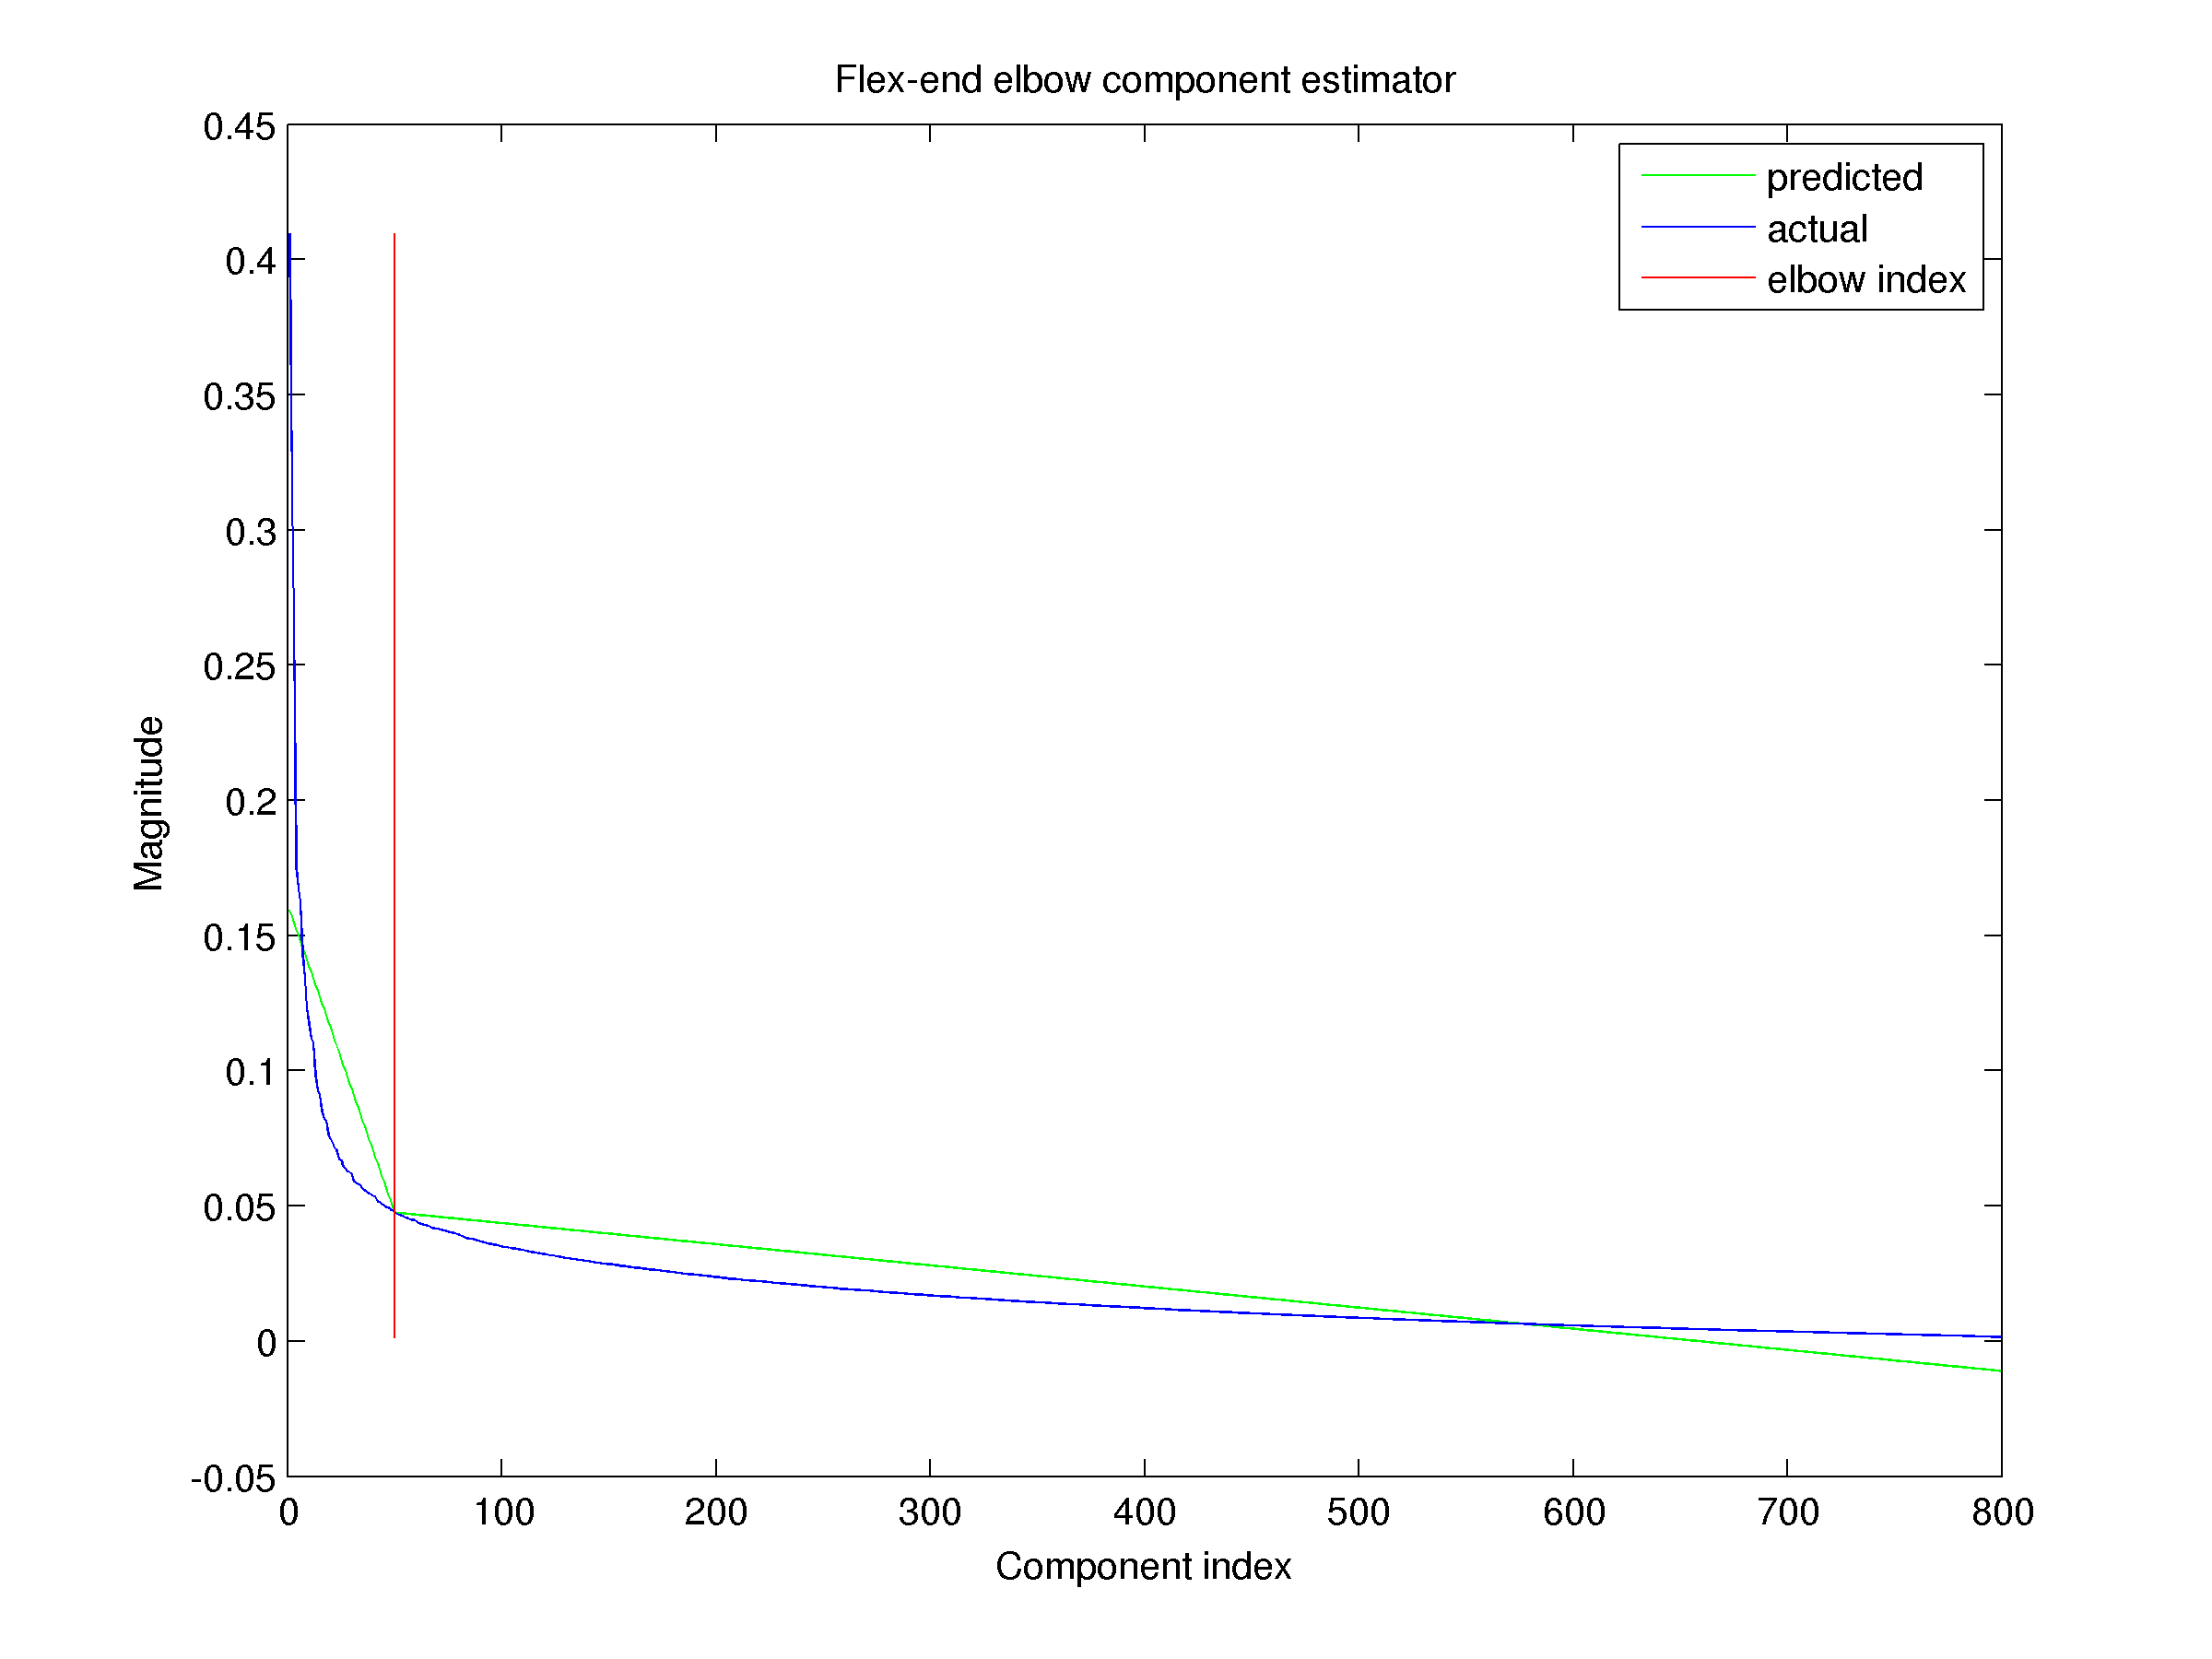
\includegraphics[width=0.9\linewidth]{2797words-adj-800dim-lowercase-wmt-model-original-flex_end_elbow}
    \caption{Eigenvalues for each principal component of the 1860 word vectors
    produced from the 2797 word list.}
    \label{fig:2797wordsunnormalizedpcaeigenvalues}
\end{figure}

Table \ref{tab:2797wordsRankingsUnnormalizedPCA} gives the highest and lowest
ranking words on the first 4 principal components of the unnormalized 1860 word 
vectors. A more complete list can be found in Appendix 
\ref{app:rankedwordlists:2797words:unnormalized}.


\subsection{Normalized PCA}

\begin{longtable}[tbp]{| rllll |}
    \hline
      & \multicolumn{4}{c|}{\textbf{Component}} \\
    \textbf{Rank} & \textbf{1} & \textbf{2} & \textbf{3} & \textbf{4} \\
    \endhead
    \hline
    1 & stringent\_jj  & warm\_jj  & considerate\_jj  & objector \\
    2 & beneficial\_jj  & elegant\_jj  & sociable\_jj  & loyal\_jj \\
    3 & indirect\_jj  & savant  & courteous\_jj  & staunch\_jj \\
    4 & contentious\_jj  & vibrant\_jj  & trustworthy\_jj  & devout\_jj \\
    5 & dependent\_jj  & luxurious\_jj  & articulate\_jj  & avid\_jj \\
    6 & prudent\_jj  & sparkling\_jj  & open-minded\_jj  & sociable\_jj \\
    7 & lax\_jj  & graceful\_jj  & approachable\_jj  & alcoholic \\
    \hline
    1854 & guileless\_jj  & inhuman\_jj  & bendable\_jj  & oblique\_jj \\
    1855 & sardonic\_jj  & slanderous\_jj  & soft-shelled\_jj  & contrived\_jj \\
    1856 & self-possessed\_jj  & deceitful\_jj  & broiler  & imprecise\_jj \\
    1857 & go-getter  & untruthful\_jj  & butterfly  & dissonant\_jj \\
    1858 & girlish\_jj  & cowardly\_jj  & pixy  & defamatory\_jj \\
    1859 & vivacious\_jj  & bigoted\_jj  & comforter  & limpid\_jj \\
    1860 & mousy\_jj  & defamatory\_jj  & gingery\_jj  & unvarying\_jj \\
    \hline
    \caption{The highest and lowest ranking words on the first 4 components 
    derived from normalized PCA of the 1860 word vectors 
    derived from the 2797 word list.} 
    \label{tab:2797wordsRankingsNormalizedPCA}
\end{longtable}


\begin{figure}[!tbp]
    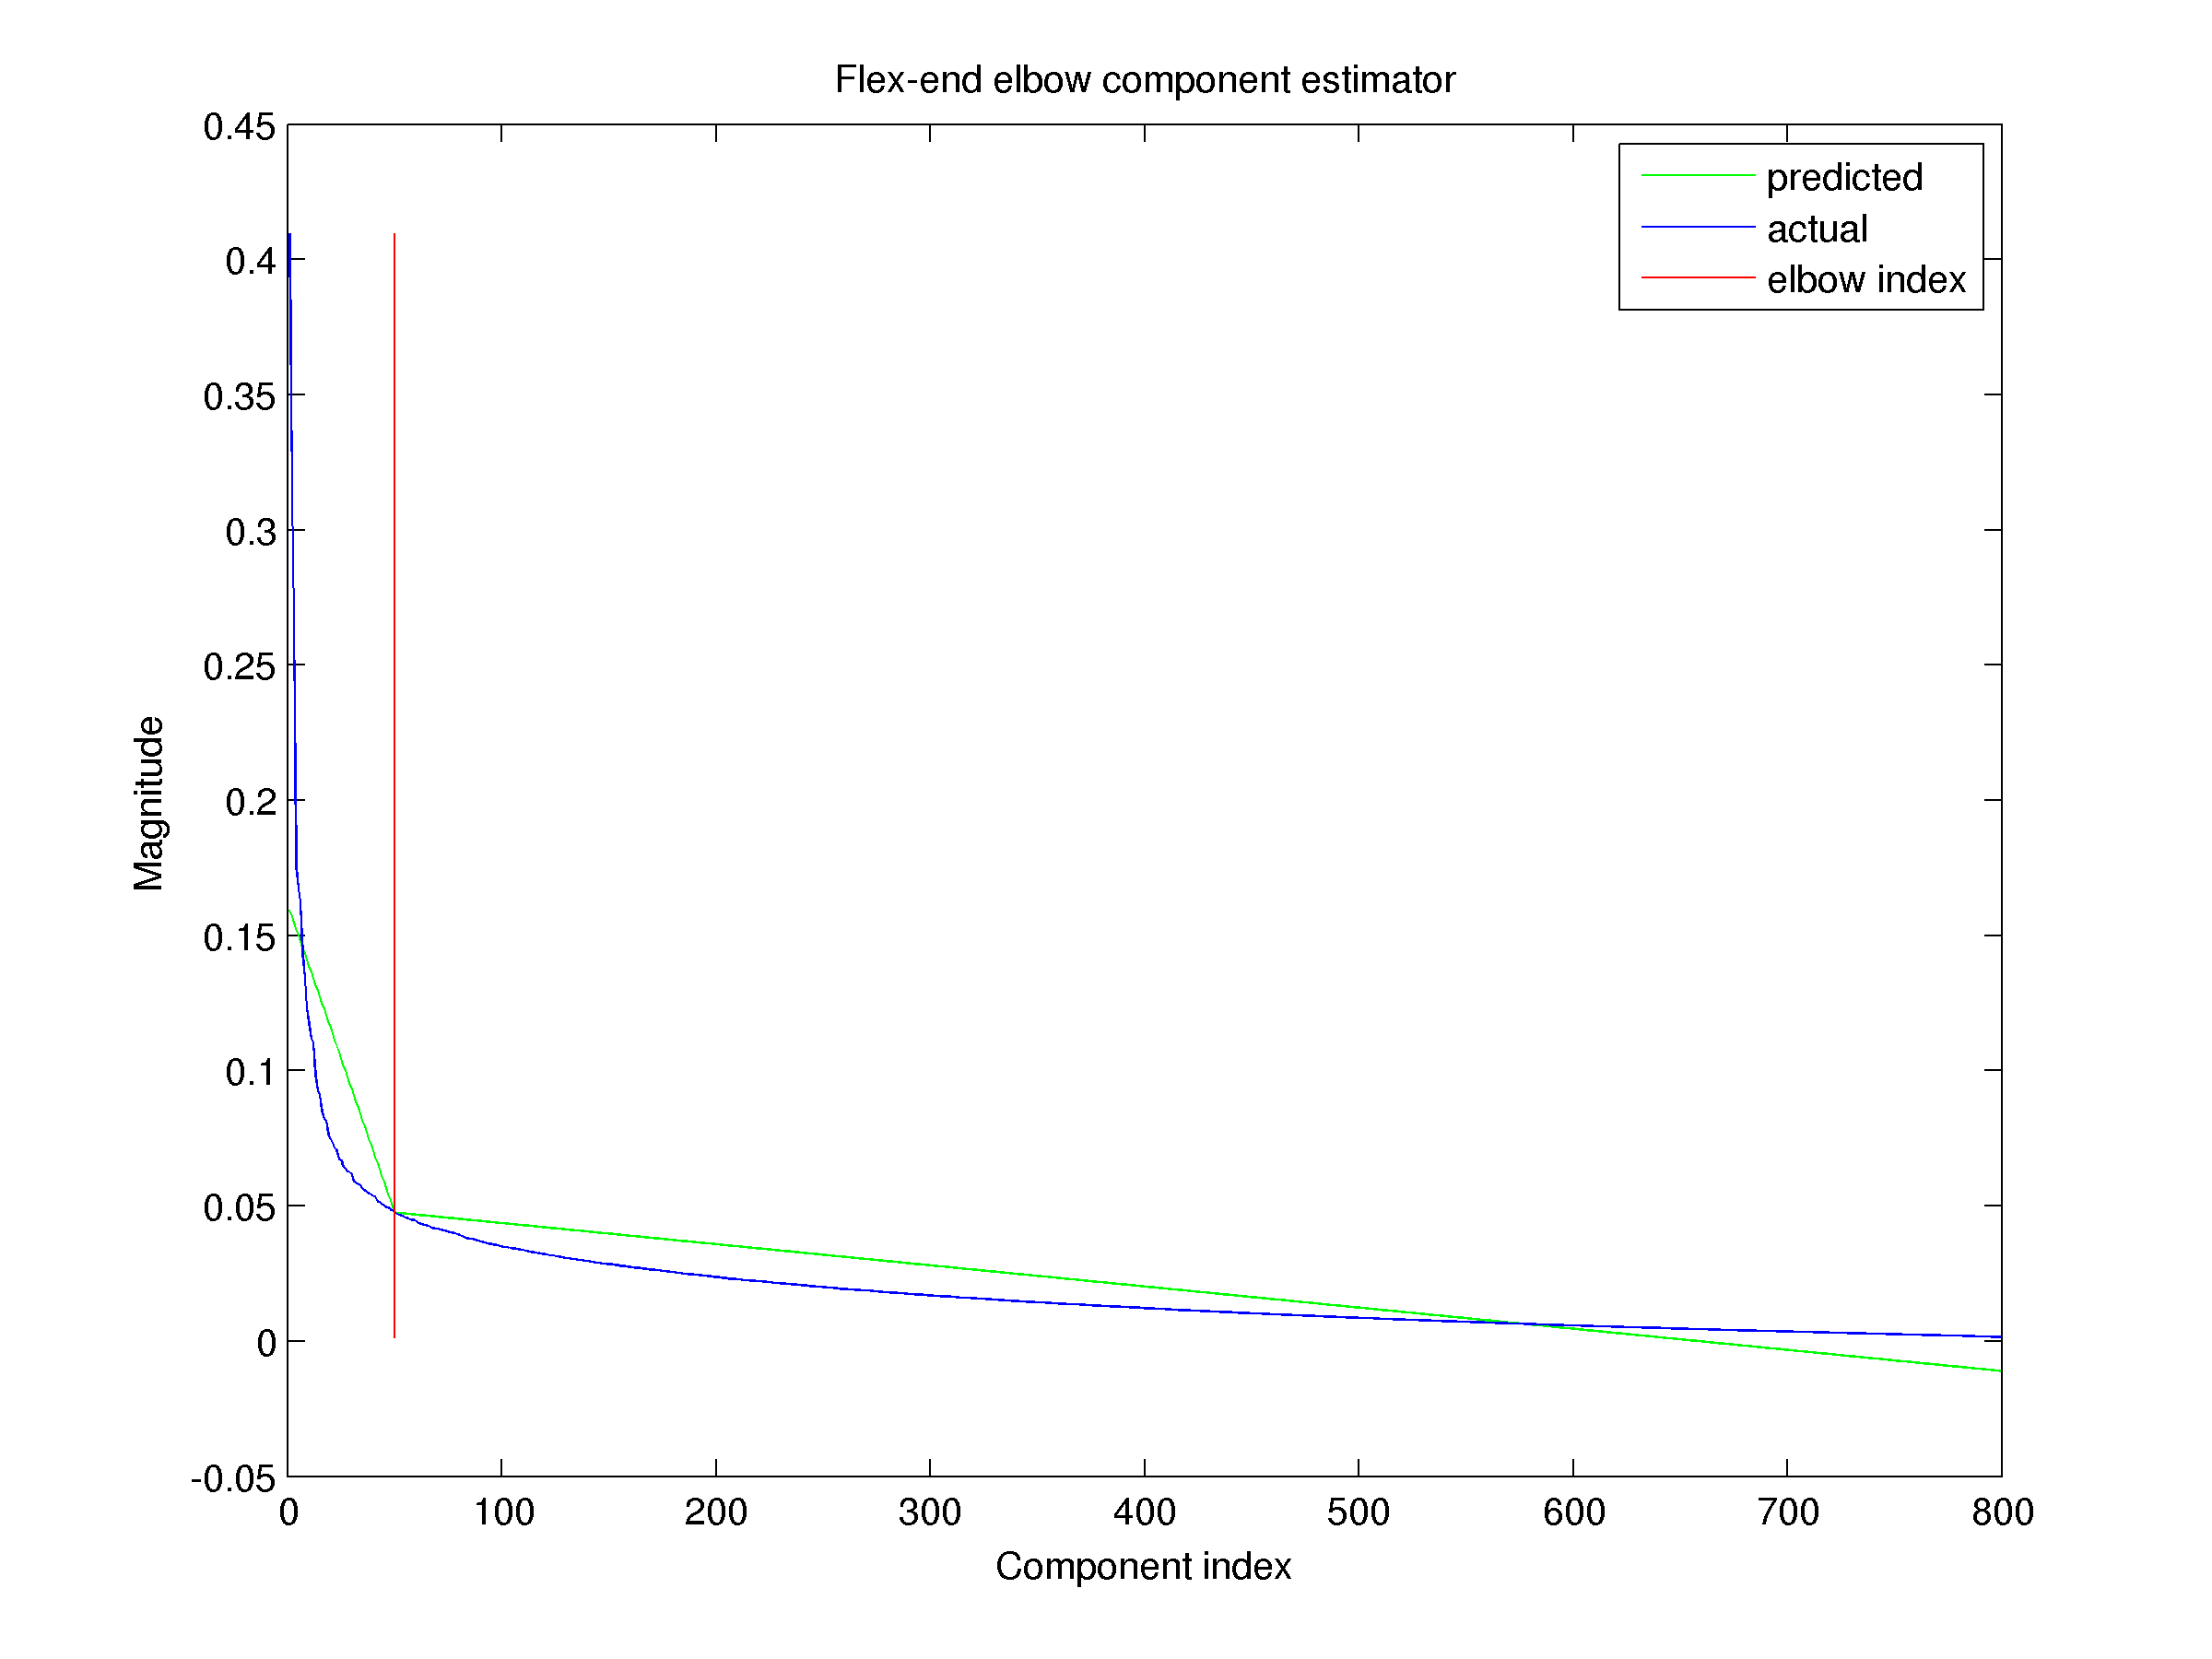
\includegraphics[width=0.9\linewidth]{2797words-adj-800dim-lowercase-wmt-model-original-flex_end_elbow}
    \caption{Eigenvalues for each principal component of the 1860 z-score 
    normalized word vectors produced from the 2797 word list.}
    \label{fig:2797wordsnormalizedpcaeigenvalues}
\end{figure}

Table \ref{tab:2797wordsRankingsNormalizedPCA} gives the highest and lowest
ranking words on the first 4 principal components of the z-score normalized 1860
word vectors. A more complete list can be found in Appendix 
\ref{app:rankedwordlists:2797words:normalized}.

\subsection{MDS}

\begin{longtable}[!htbp]{| rllll |}
    \hline
      & \multicolumn{4}{c|}{\textbf{Component}} \\
    \textbf{Rank} & \textbf{1} & \textbf{2} & \textbf{3} & \textbf{4} \\
    \endhead
    \hline
    1 & gamin  & bigoted\_jj  & thoughtful\_jj  & fan \\
    2 & coquettish\_jj  & unethical\_jj  & honest\_jj  & lucky\_jj \\
    3 & kittenish\_jj  & hypocritical\_jj  & pragmatic\_jj  & staunch\_jj \\
    4 & tender-hearted\_jj  & untruthful\_jj  & trustworthy\_jj  & bulldog \\
    5 & shrewish\_jj  & godless\_jj  & open-minded\_jj  & rowdy\_jj \\
    6 & donnish\_jj  & untransparent\_jj  & forthright\_jj  & stalwart \\
    7 & slangy\_jj  & dishonest\_jj  & articulate\_jj  & jealous\_jj \\
    \hline
    1854 & direct\_jj  & sunny\_jj  & yellow\_jj  & poetic\_jj \\
    1855 & reasonable\_jj  & polished\_jj  & butterfly  & imaginative\_jj \\
    1856 & consistent\_jj  & elegant\_jj  & gingery\_jj  & recondite\_jj \\
    1857 & contentious\_jj  & vibrant\_jj  & bendable\_jj  & assimilative\_jj \\
    1858 & prudent\_jj  & calm\_jj  & broiler  & participative\_jj \\
    1859 & stringent\_jj  & graceful\_jj  & pixy  & undogmatic\_jj \\
    1860 & beneficial\_jj  & lively\_jj  & soft-shelled\_jj  & abstract\_jj \\
    \hline
    \caption{\todo{need to caption the table for 2797words-adj-800dim-lowercase-wmt-model-mds-transformed-summary-table.tex} } \\
\end{longtable}


Table \ref{tab:2797wordsRankingsMDS} gives the highest and lowest
ranking words on the first 4 principal components of the 1860 word 
vectors after MDS. A more complete list can be found in Appendix 
\ref{app:rankedwordlists:2797words:mds}.

\begin{figure}[!tbp]
    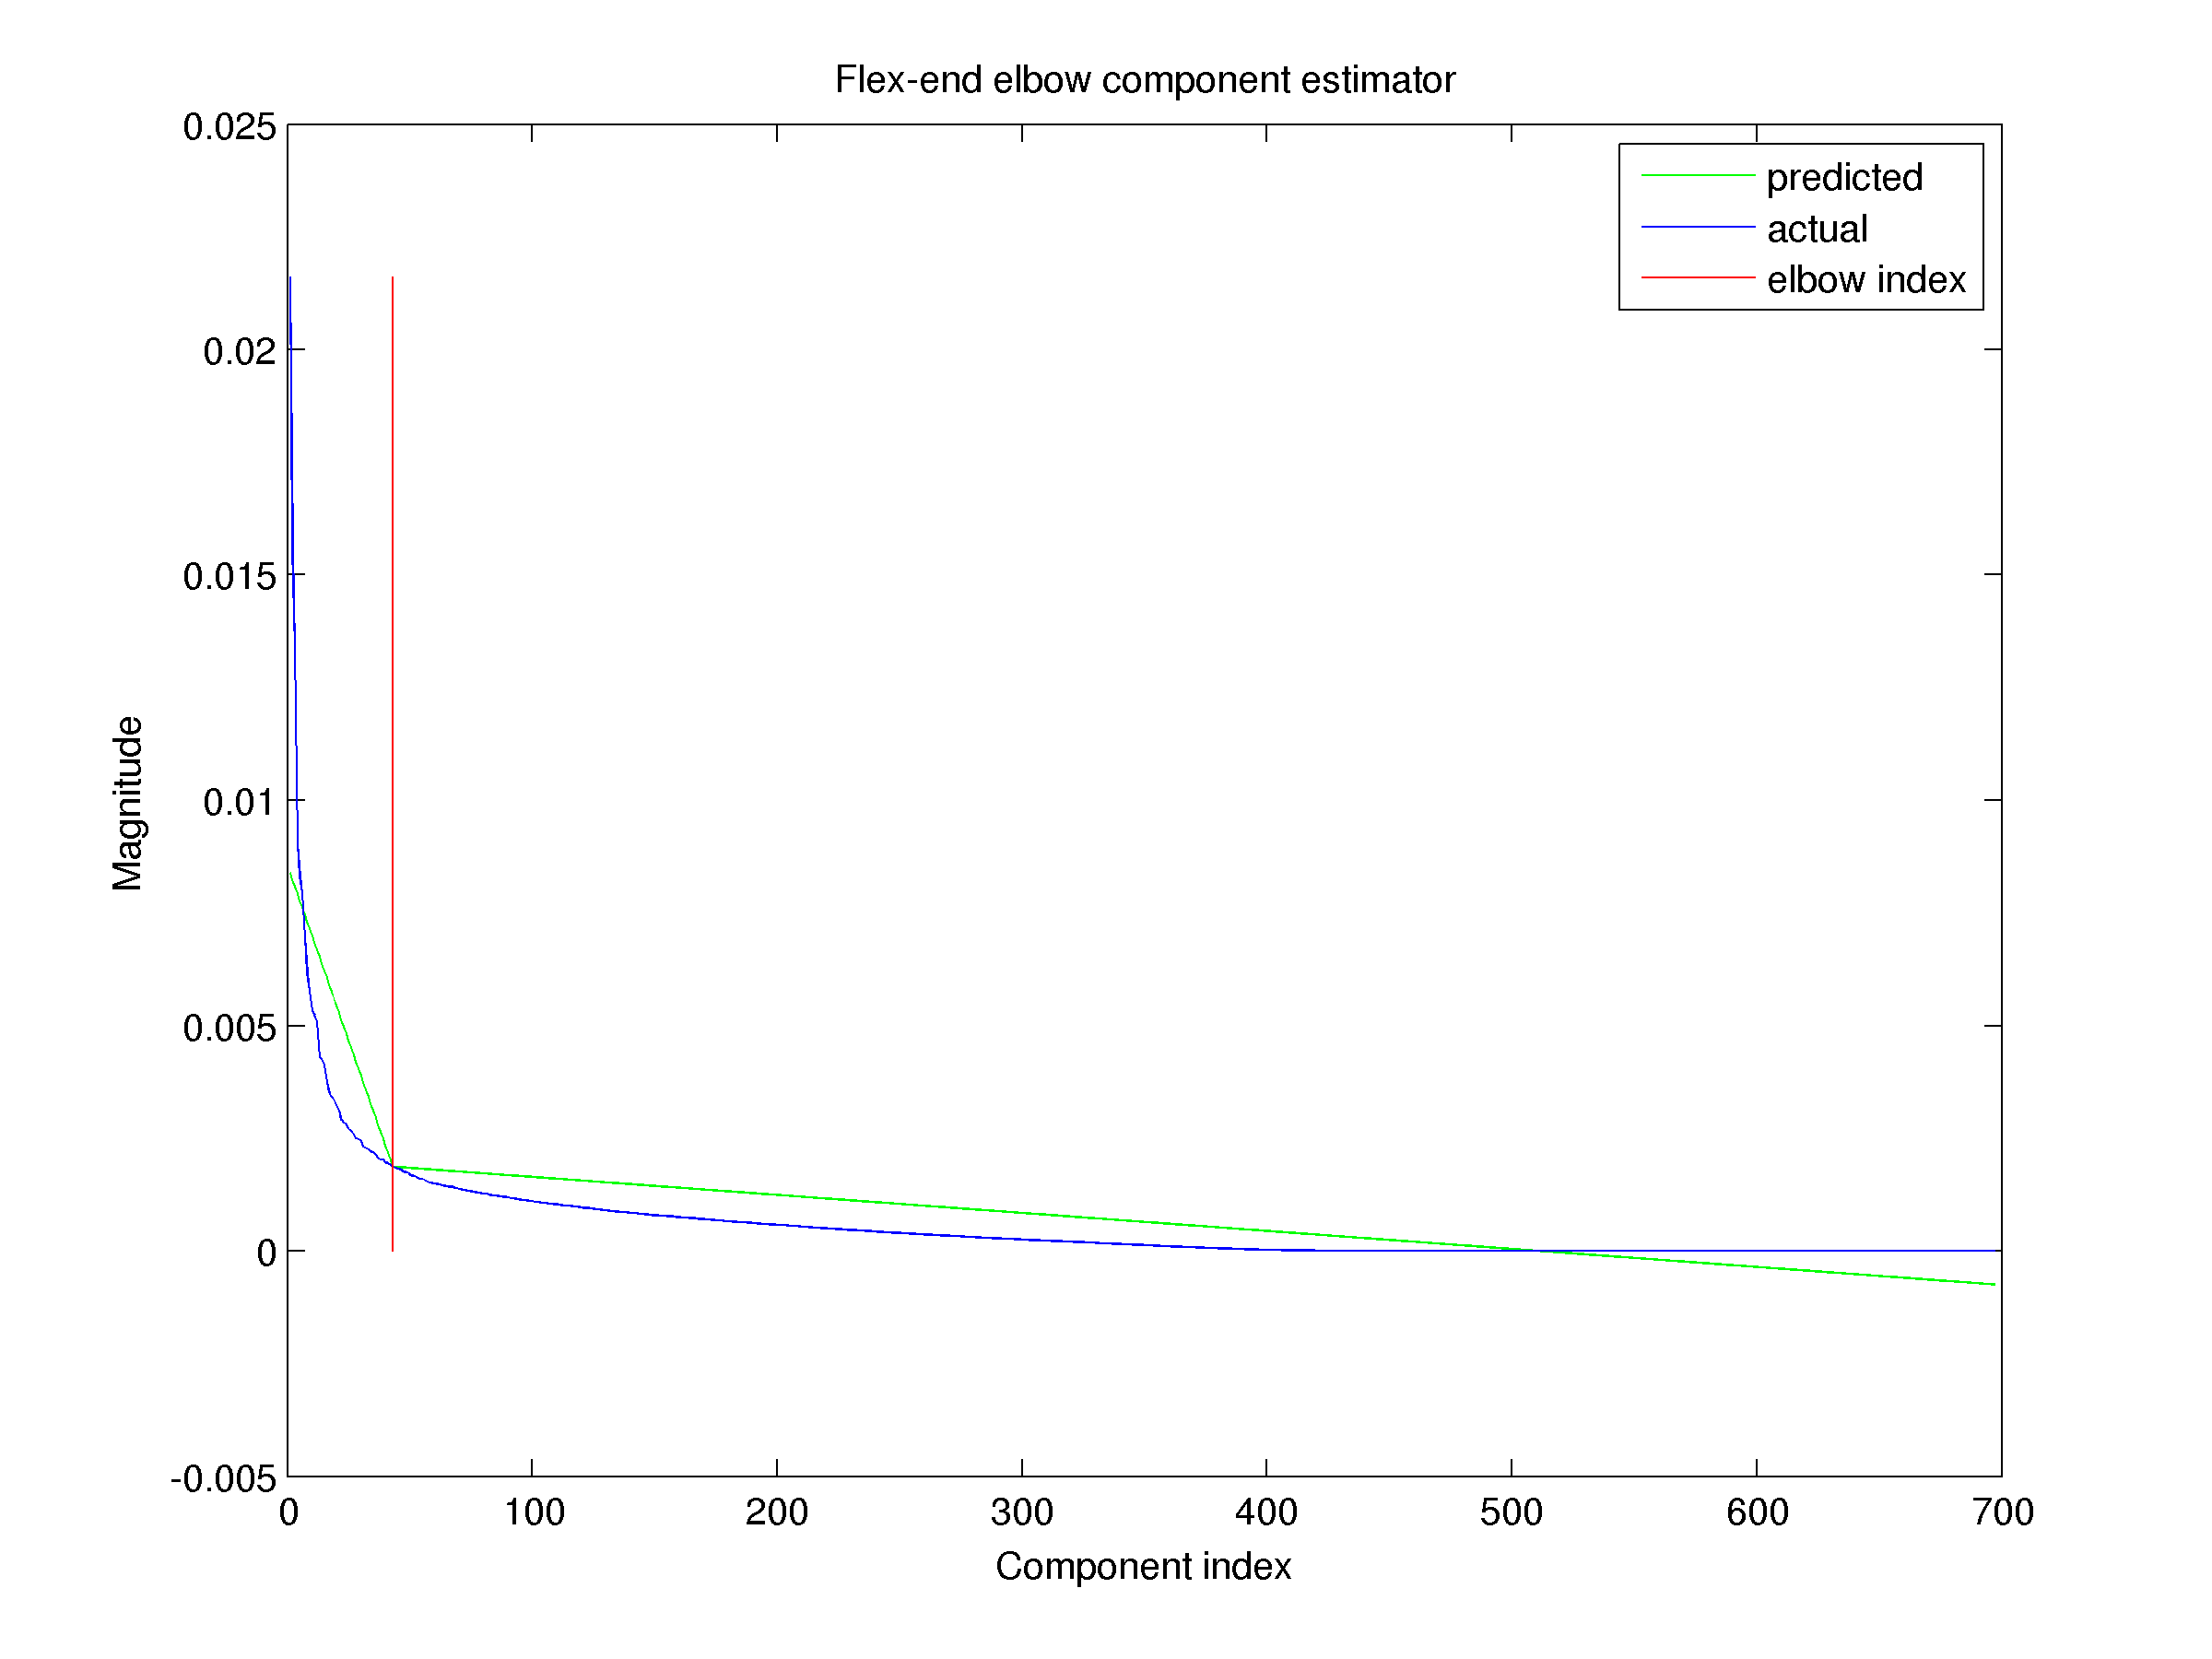
\includegraphics[width=0.9\linewidth]{2797words-adj-800dim-lowercase-wmt-model-mds-transformed-flex_end_elbow}
    \caption{Eigenvalues for each principal component of the 1860 word vectors
    produced from the 2797 word list after multidimensional scaling.}
    \label{fig:2797wordsmdseigenvalues}
\end{figure}


\section{Combined 2797, 438, and 101 word sets}

When the three word-lists are combined, it adds another 118 words, for 1978
total. The additional words are listed in Table 
\ref{additionalwordsin2797combined}. Since they make up 6\% of the resulting
list, these have more effect on the resulting
components than adding 9 vectors to the 421 vectors from the 439 word list.
However, as Figure \ref{fig:2797vs2797and439and100} shows, they are still
extremely close. See Appendix \ref{app:rankedwordlists:2797and438and101words}
the ranked word lists.


\begin{figure}[!tbp]
    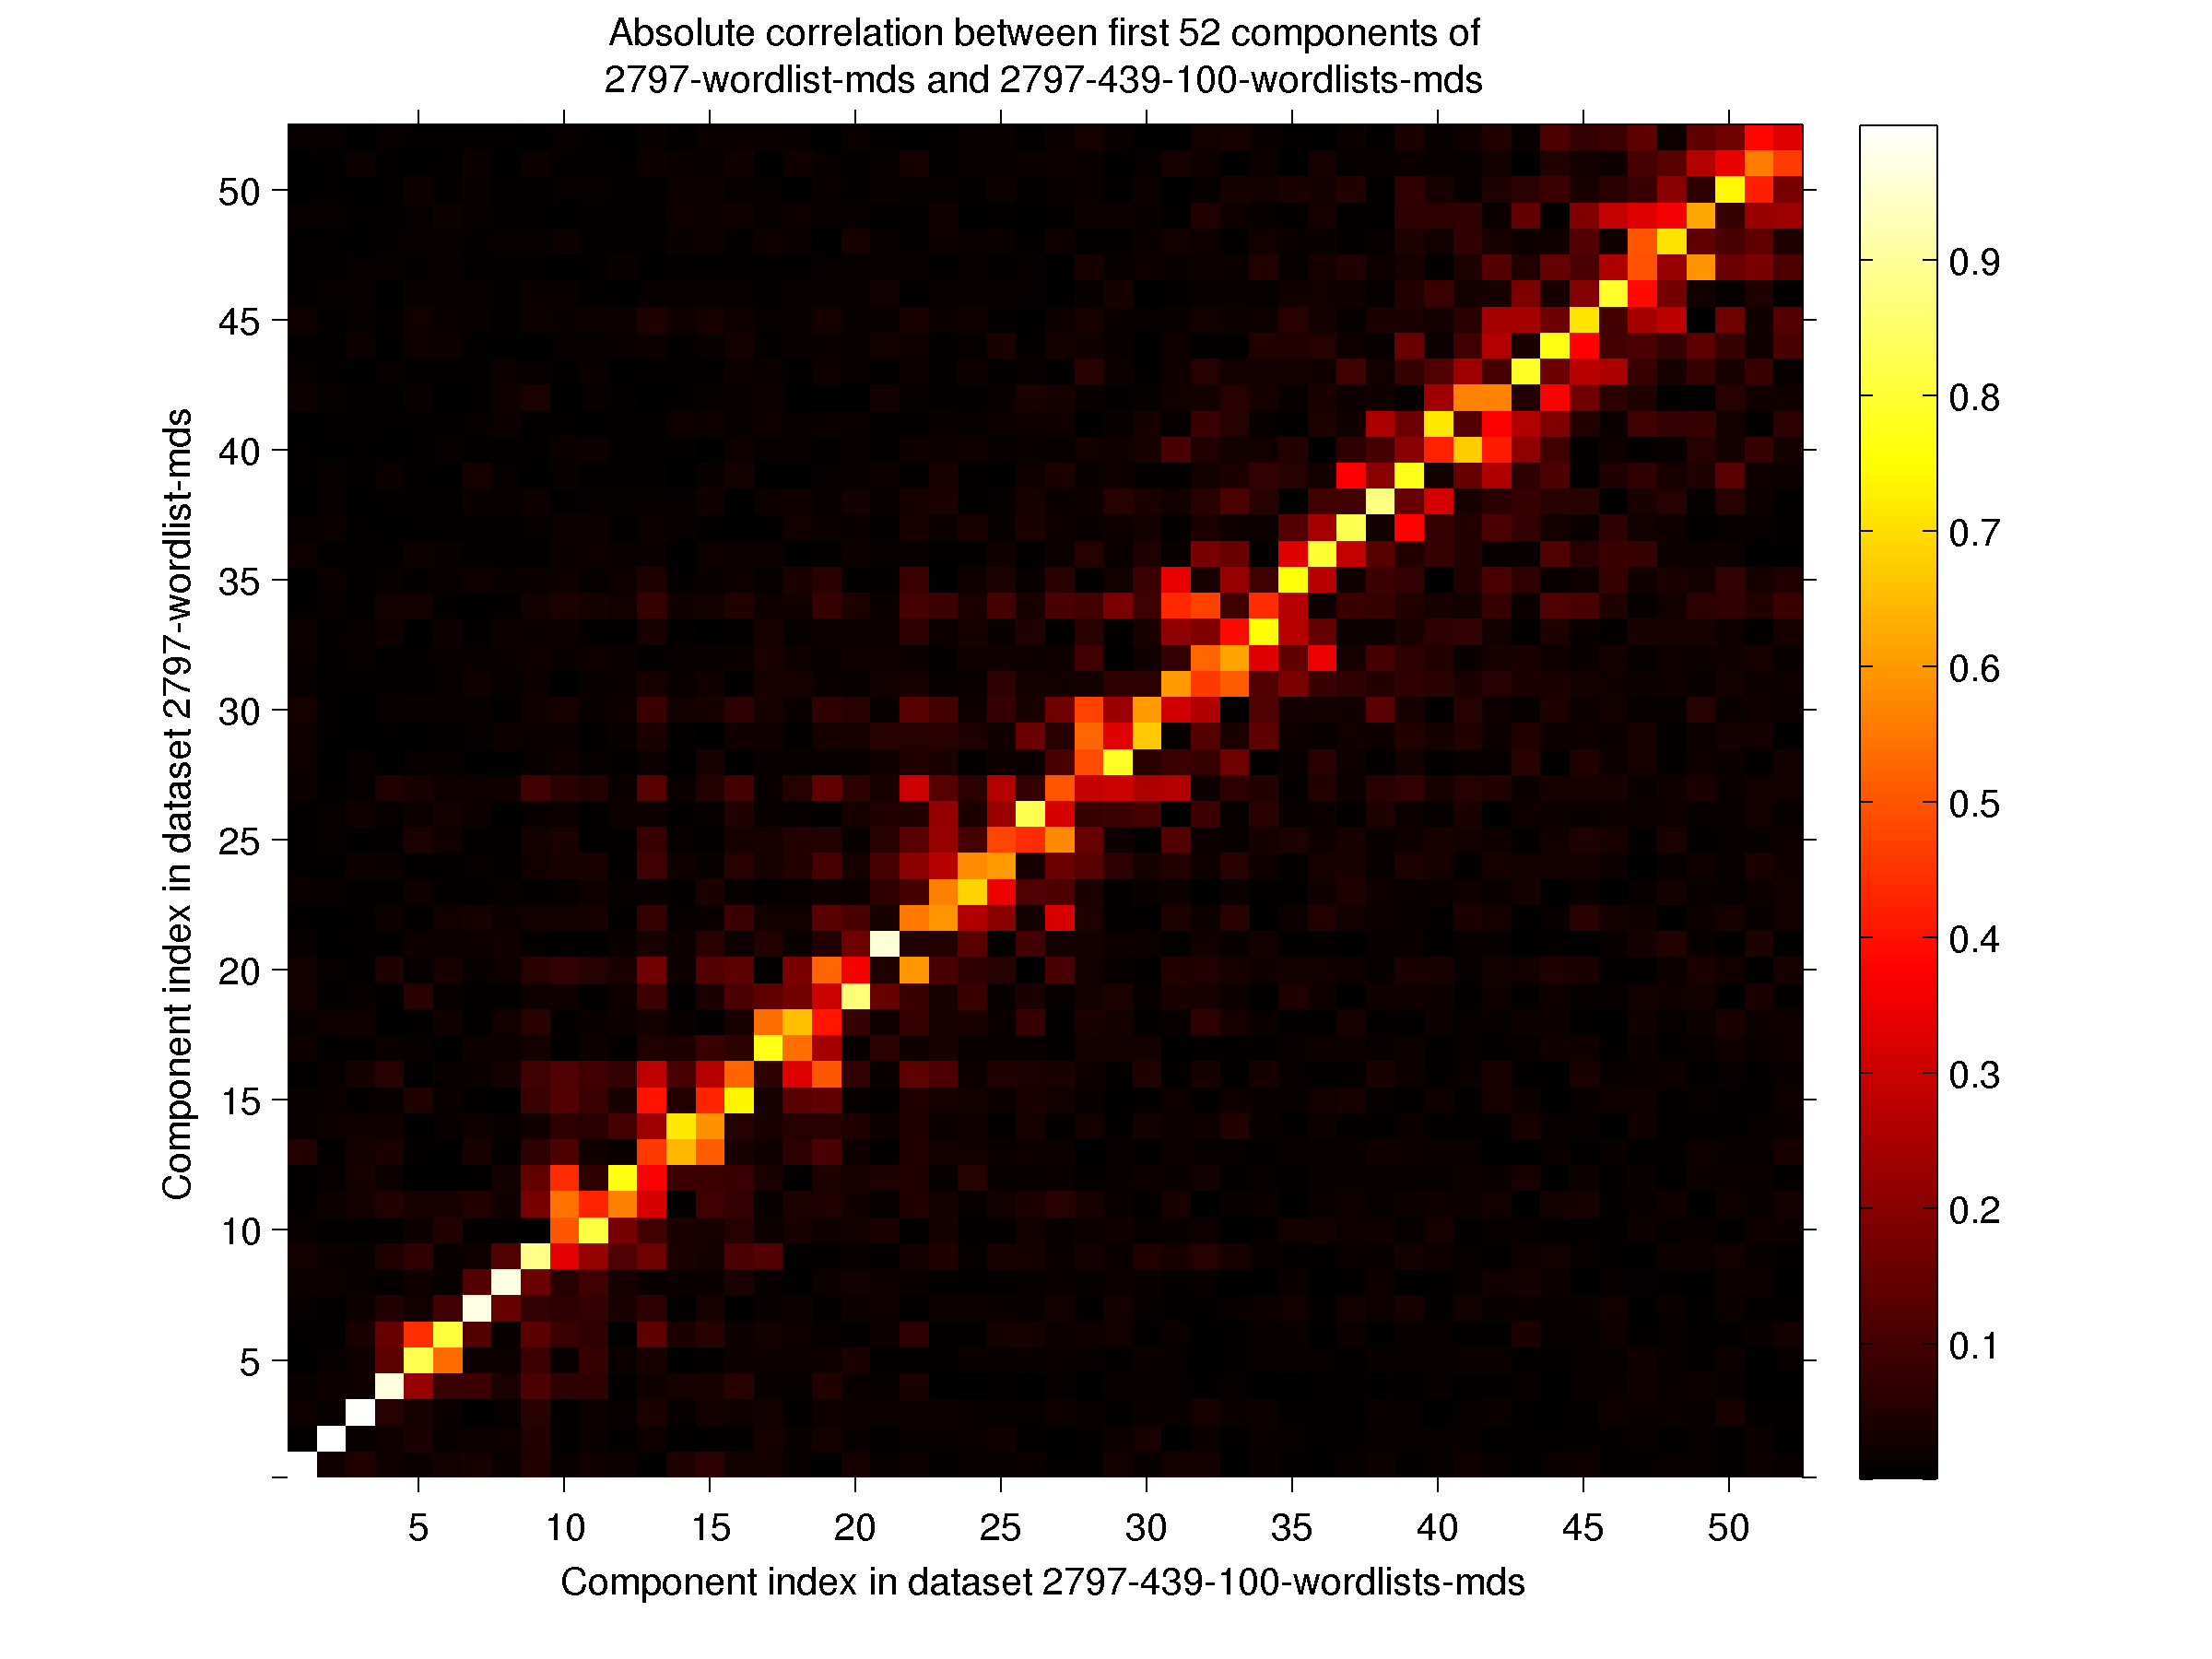
\includegraphics[width=0.9\linewidth]{2797-vs-2797and439and1100-from-800dim-lowercase-wmt-model-correlations}
    \caption{Correlations between the first 52 MDS vectors generated from the 
    2797 word list alone and the first 52 vectors generated from the combined
    2797 word, 439 word and 101 word lists.}
    \label{fig:2797vs2797and439and100}
\end{figure}


\begin{table}[tbp]
    \begin{tabular}{| llll |}
        \hline
        aimlessness & aloofness & ambition & amiability \\
        animation & anxious\_jj & assertion & belligerence \\
        bossiness & callousness & candor & caution \\
        conceit & conventionality & cooperation & courage \\
        courtesy & creativity & cruelty & curiosity \\
        deceit & decisiveness & defensive\_jj & demanding\_jj \\
        dependability & depth & dignity & disorganization \\
        distrust & dominant\_jj & dull\_jj & earthiness \\
        easygoing\_jj & efficiency & egotistical\_jj & emotionality \\
        empathy & enthusiastic\_jj & envious\_jj & envy \\
        erratic\_jj & exhibitionistic\_jj & expressiveness & fear \\
        fearful\_jj & flexibility & forgetfulness & frivolity \\
        generosity & gregariousness & gullibility & humor \\
        humorous\_jj & inconsistency & indecisiveness & independence \\
        inhibition & insecurity & insight & instability \\
        intellectuality & intelligence & intrusiveness & irritability \\
        leniency & lethargy & logic & modest\_jj \\
        modesty & morality & naïve\_jj & natural\_jj \\
        naturalness & negligence & nonconformity & opportunistic\_jj \\
        optimism & organization & organized\_jj & passivity \\
        persistence & pessimism & placidity & playfulness \\
        pomposity & precision & predictability & prejudice \\
        prejudiced\_jj & punctuality & quiet & recklessness \\
        reserve & rudeness & self-esteem & selfishness \\
        shallowness & shyness & silence & simple\_jj \\
        sloth & smart\_jj & sophistication & spirit \\
        spontaneity & stinginess & stubbornness & stupidity \\
        surliness & talkativeness & thoughtlessness & thrift \\
        underhanded\_jj & understanding & unfriendliness & volatility \\
        warmth & neat\_jj &  &  \\
        \hline
    \end{tabular}
    \caption{The 181 words not present in the 1860 word vectors derived from
    the tagged 2797 word list}
    \label{tab:additionalwordsin2797combined}

\end{table}



\section{Dimension Matching}
\subsection{Overview}

As mentioned in the methods section \todo{reference where the dimension 
matching is mentioned in the reference section instead of saying ``in the 
methods section''}, we looked at the matches between the principal components
discovered in the different wordlists as a validation as to whether the same
semantics were being covered and as an indication of how many dimensions might 
be significant.

\subsection{439 and 100 vs 2797}

We began our comparison of the various dimensions with a comparison of all 
components of the combined 439 and 100 word datasets with all of the components
of the 2797 word dataset. There is a pretty dense collection of matches at
dimension less than 52 in the 2797 word list. See Figure 
\ref{fig:439and100vs2797} and Table
\ref{439and100-vs-2797-from-800dim-lowercase-wmt-model-significant.tex}. 

\begin{table}[!tbp]
    \begin{tabular}{| p{0.75in}p{3.5in} |}
        \hline
        \textbf{439-and-100-wordlists-combined-mds dim} & \textbf{2797-wordlist-mds -- dim(correlation)}\\
        1 & 1(0.95), 3(0.33)\\
        2 & 2(-0.88), 3(0.32), 5(-0.34)\\
        3 & 2(0.65), 3(0.32), 4(0.42), 6(0.5), 16(0.29)\\
        4 & 4(-0.53), 7(0.54), 8(-0.46)\\
        5 & 3(-0.47), 4(-0.47), 7(-0.43), 8(-0.36), 10(0.37), 11(-0.35), 13(-0.3), 25(-0.31)\\
        6 & 5(-0.81), 11(-0.33), 18(0.3)\\
        7 & 4(0.32), 8(-0.47), 9(0.51), 12(0.36), 14(0.33)\\
        8 & 6(0.66), 7(0.31), 11(0.3)\\
        9 & 3(0.34), 4(-0.33), 6(0.29), 12(0.49), 14(0.4)\\
        10 & 8(0.47), 9(0.49)\\
        11 & 6(-0.31), 10(-0.59)\\
        12 & 7(0.33), 11(-0.43), 14(0.34)\\
        13 & 15(-0.4), 17(-0.43), 18(0.3), 21(0.39), 22(-0.43), 23(-0.33)\\
        14 & 11(0.4), 14(0.37)\\
        15 & 13(-0.56), 28(0.3)\\
        16 & 20(0.33), 24(0.29), 26(-0.3), 29(-0.38), 33(-0.29)\\
        18 & 15(-0.36), 19(0.36), 32(-0.3)\\
        19 & 16(-0.51), 41(0.29)\\
        20 & 26(0.3), 35(-0.37)\\
        21 & 17(-0.31), 19(0.29), 22(0.3)\\
        23 & 12(0.31), 20(0.31)\\
        24 & 23(-0.28), 40(0.34)\\
        25 & 39(0.3)\\
        26 & 35(0.29)\\
        27 & 29(-0.35)\\
        29 & 32(0.31)\\
        30 & 34(-0.4)\\
        31 & 112(-0.3)\\
        32 & 52(0.29)\\
        34 & 27(-0.3)\\
        35 & 74(0.3)\\
        37 & 37(0.3)\\
        46 & 50(0.31)\\
        62 & 83(0.29)\\
        66 & 93(0.3)\\
        77 & 177(0.3)\\
        81 & 178(-0.29)\\
        \hline
    \end{tabular}
    \caption{Dimensions from dataset 439-and-100-wordlists-combined-mds which had a significant correlation with a dimension from dataset 2797-wordlist-mds when all pairs of dimensions were considered with FDR controlled at 1\%. Each entry gives the matching dimension and the correlation between them.}
    \label{439and100-vs-2797-from-800dim-lowercase-wmt-model-significant.tex}
\end{table}


\begin{figure}[!tbp]
    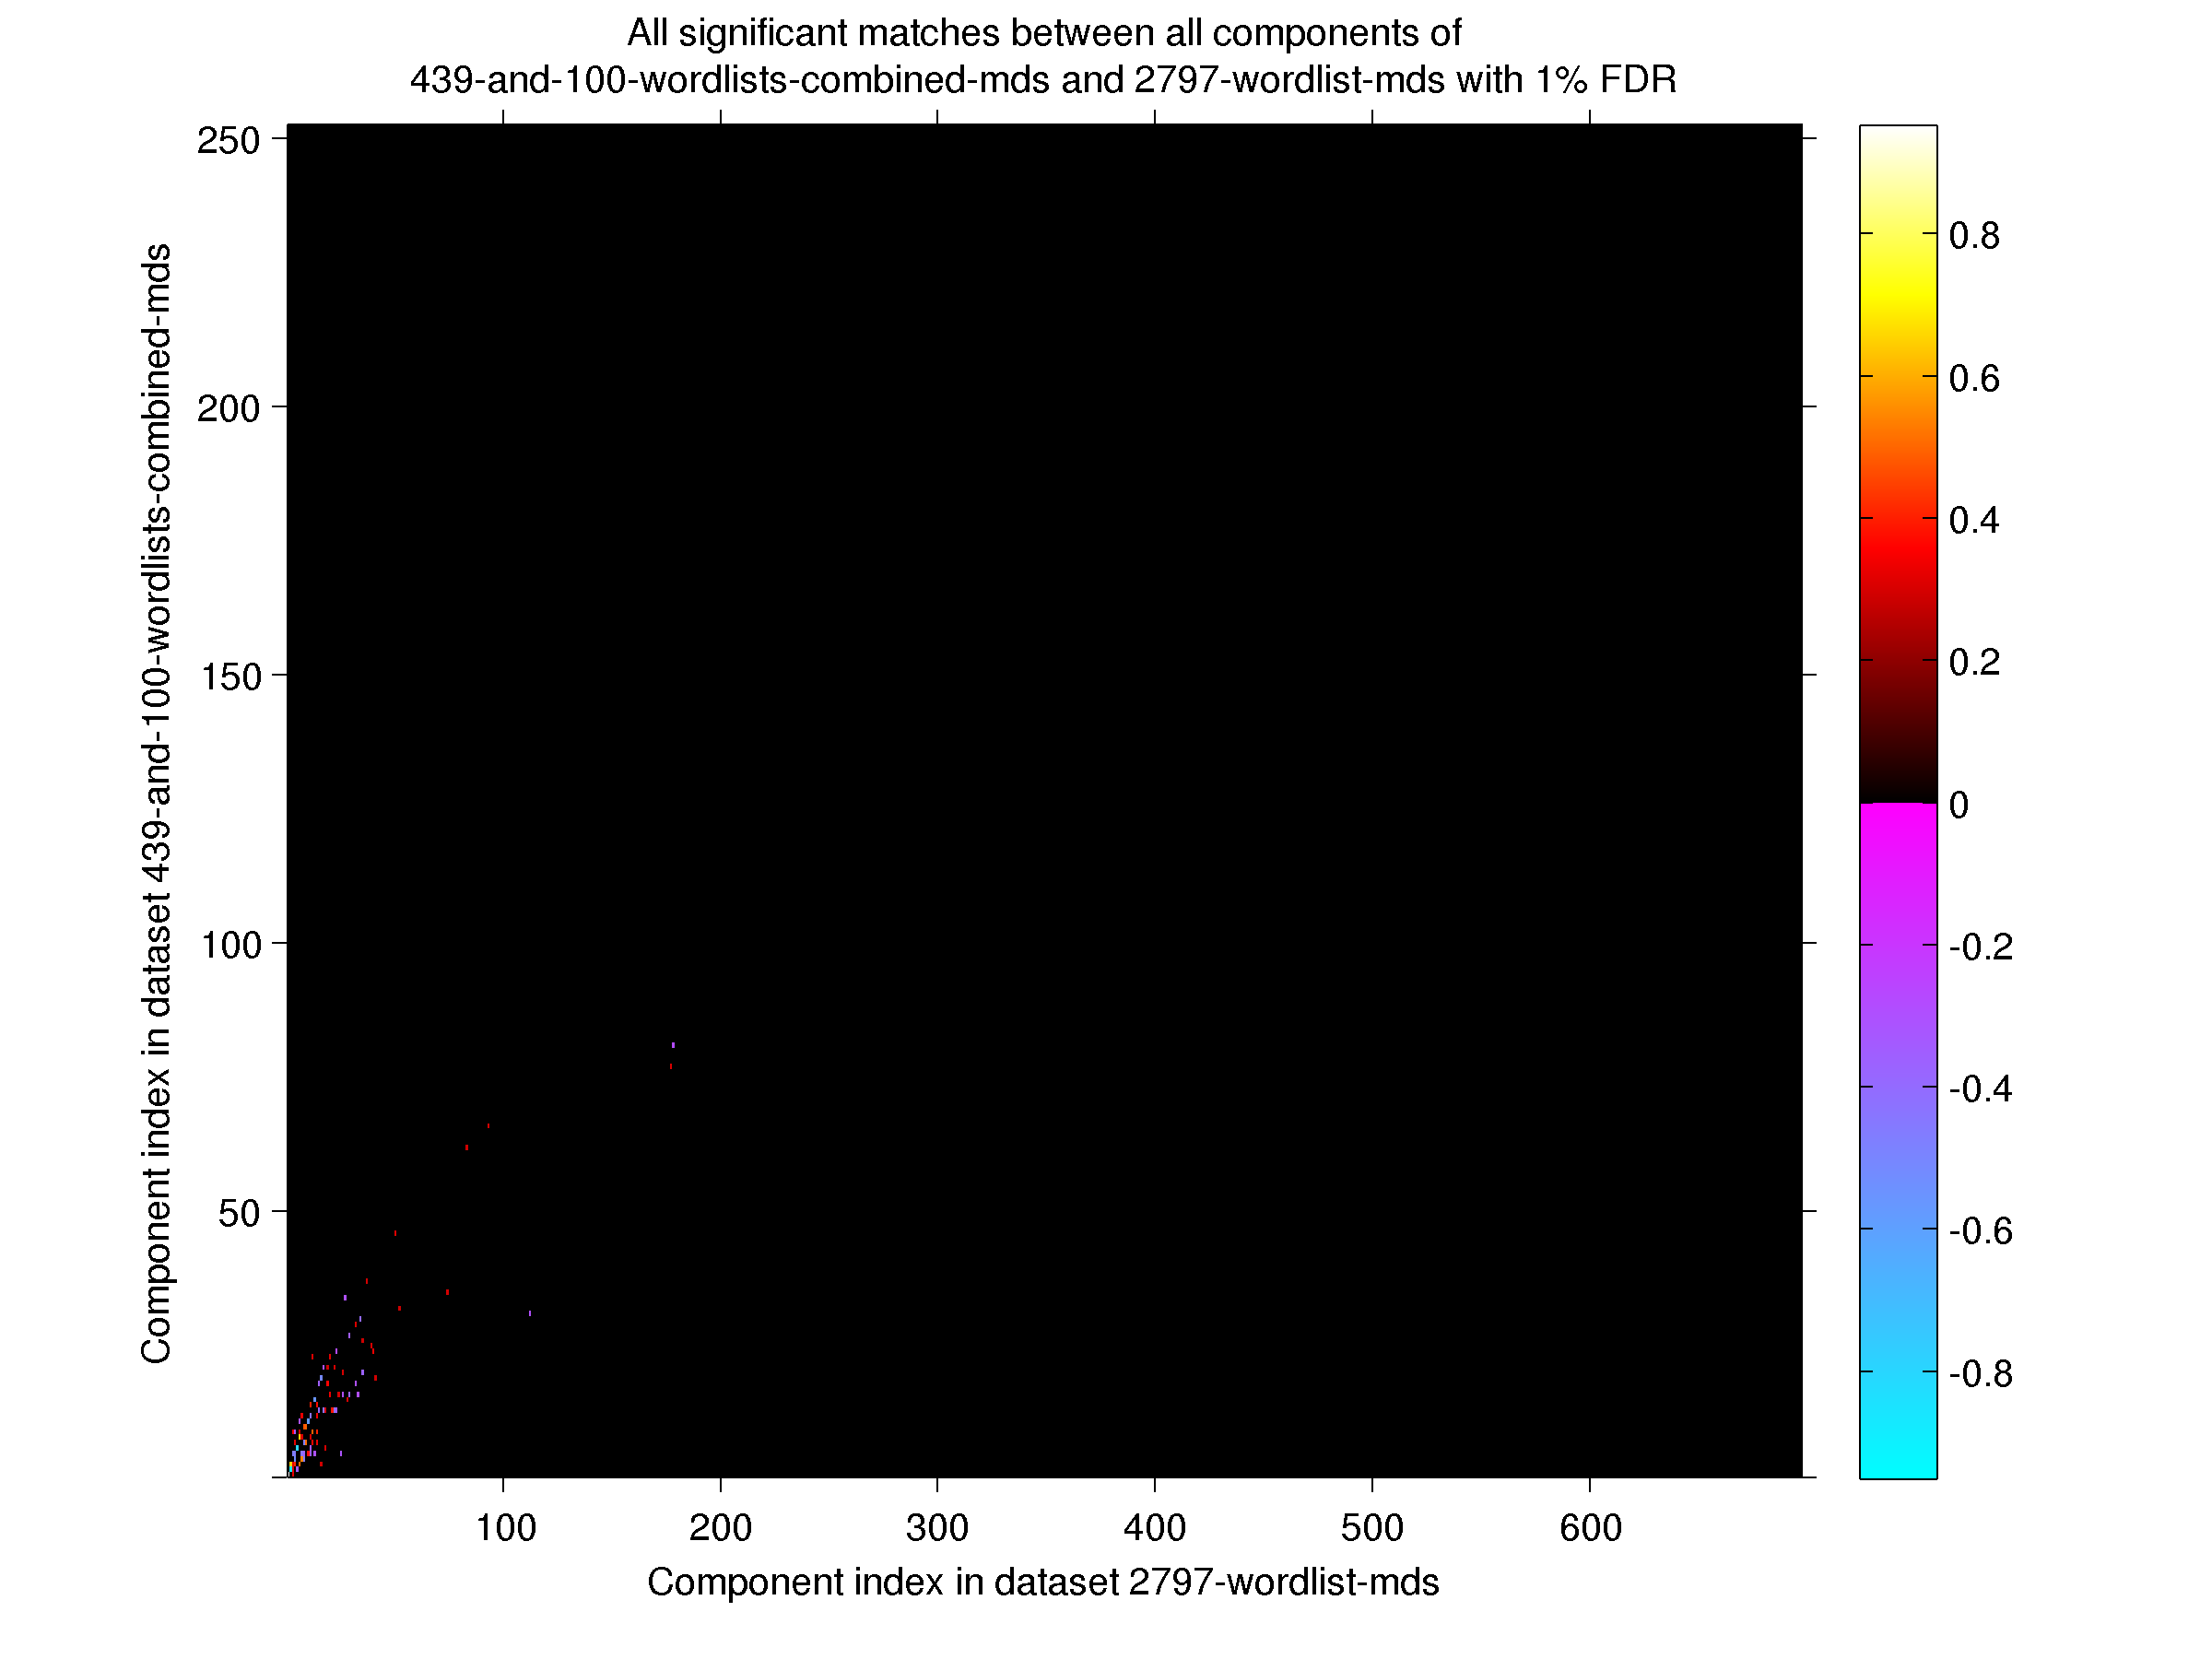
\includegraphics[width=0.9\linewidth]{439and100-vs-2797-from-800dim-lowercase-wmt-model-significant}
    \caption{Results from Table 
    \ref{439and100-vs-2797-from-800dim-lowercase-wmt-model-significant.tex} 
    displayed as an image. Colors (except black) give correlation for matching 
    dimensions.}
    \label{fig:439and100vs2797}
\end{figure}

\subsection{First 52 dimensions of 100 vs 439 and 100}

Because of the previous plot, we eliminate all but the first 52 dimensions in
looking at the components of 100 words that also appear in the combined 439
and 100 word list. This gives a relatively dense set of correspondences for the
first 22 dimensions of the combined lists (and the first 16 of the 100 word
list). See Figure \ref{fig:100vs439And100First52} and Table 
\ref{100-vs-439and100-from-800dim-lowercase-wmt-model-significant-first-52.tex}.

\begin{table}[!tbp]
    \begin{tabular}{| p{0.75in}p{3.5in} |}
        \hline
        \textbf{100-wordlist-mds dim} & \textbf{439-and-100-wordlists-combined-mds -- dim(correlation)}\\
        1 & 1(0.87), 3(0.46), 4(-0.47)\\
        2 & 2(0.87), 3(-0.56)\\
        3 & 4(0.62), 5(0.6)\\
        4 & 6(0.46), 7(-0.5), 8(-0.48)\\
        5 & 8(0.45), 11(-0.52), 13(-0.56)\\
        7 & 10(0.51)\\
        8 & 7(0.54)\\
        9 & 6(0.64)\\
        11 & 36(-0.46)\\
        12 & 10(-0.46)\\
        14 & 21(0.48), 39(-0.52)\\
        16 & 22(0.49)\\
        29 & 42(-0.47)\\
        30 & 52(0.47)\\
        \hline
    \end{tabular}
    \caption{Dimensions from dataset 100-wordlist-mds which had a significant correlation with a dimension from dataset 439-and-100-wordlists-combined-mds when only the first 52 dimensions were considered as potential matches for one another with FDR controlled at 1\%. Each entry gives the matching dimension and the correlation between them.}
    \label{100-vs-439and100-from-800dim-lowercase-wmt-model-significant-first-52.tex}
\end{table}


\begin{figure}[!tbp]
    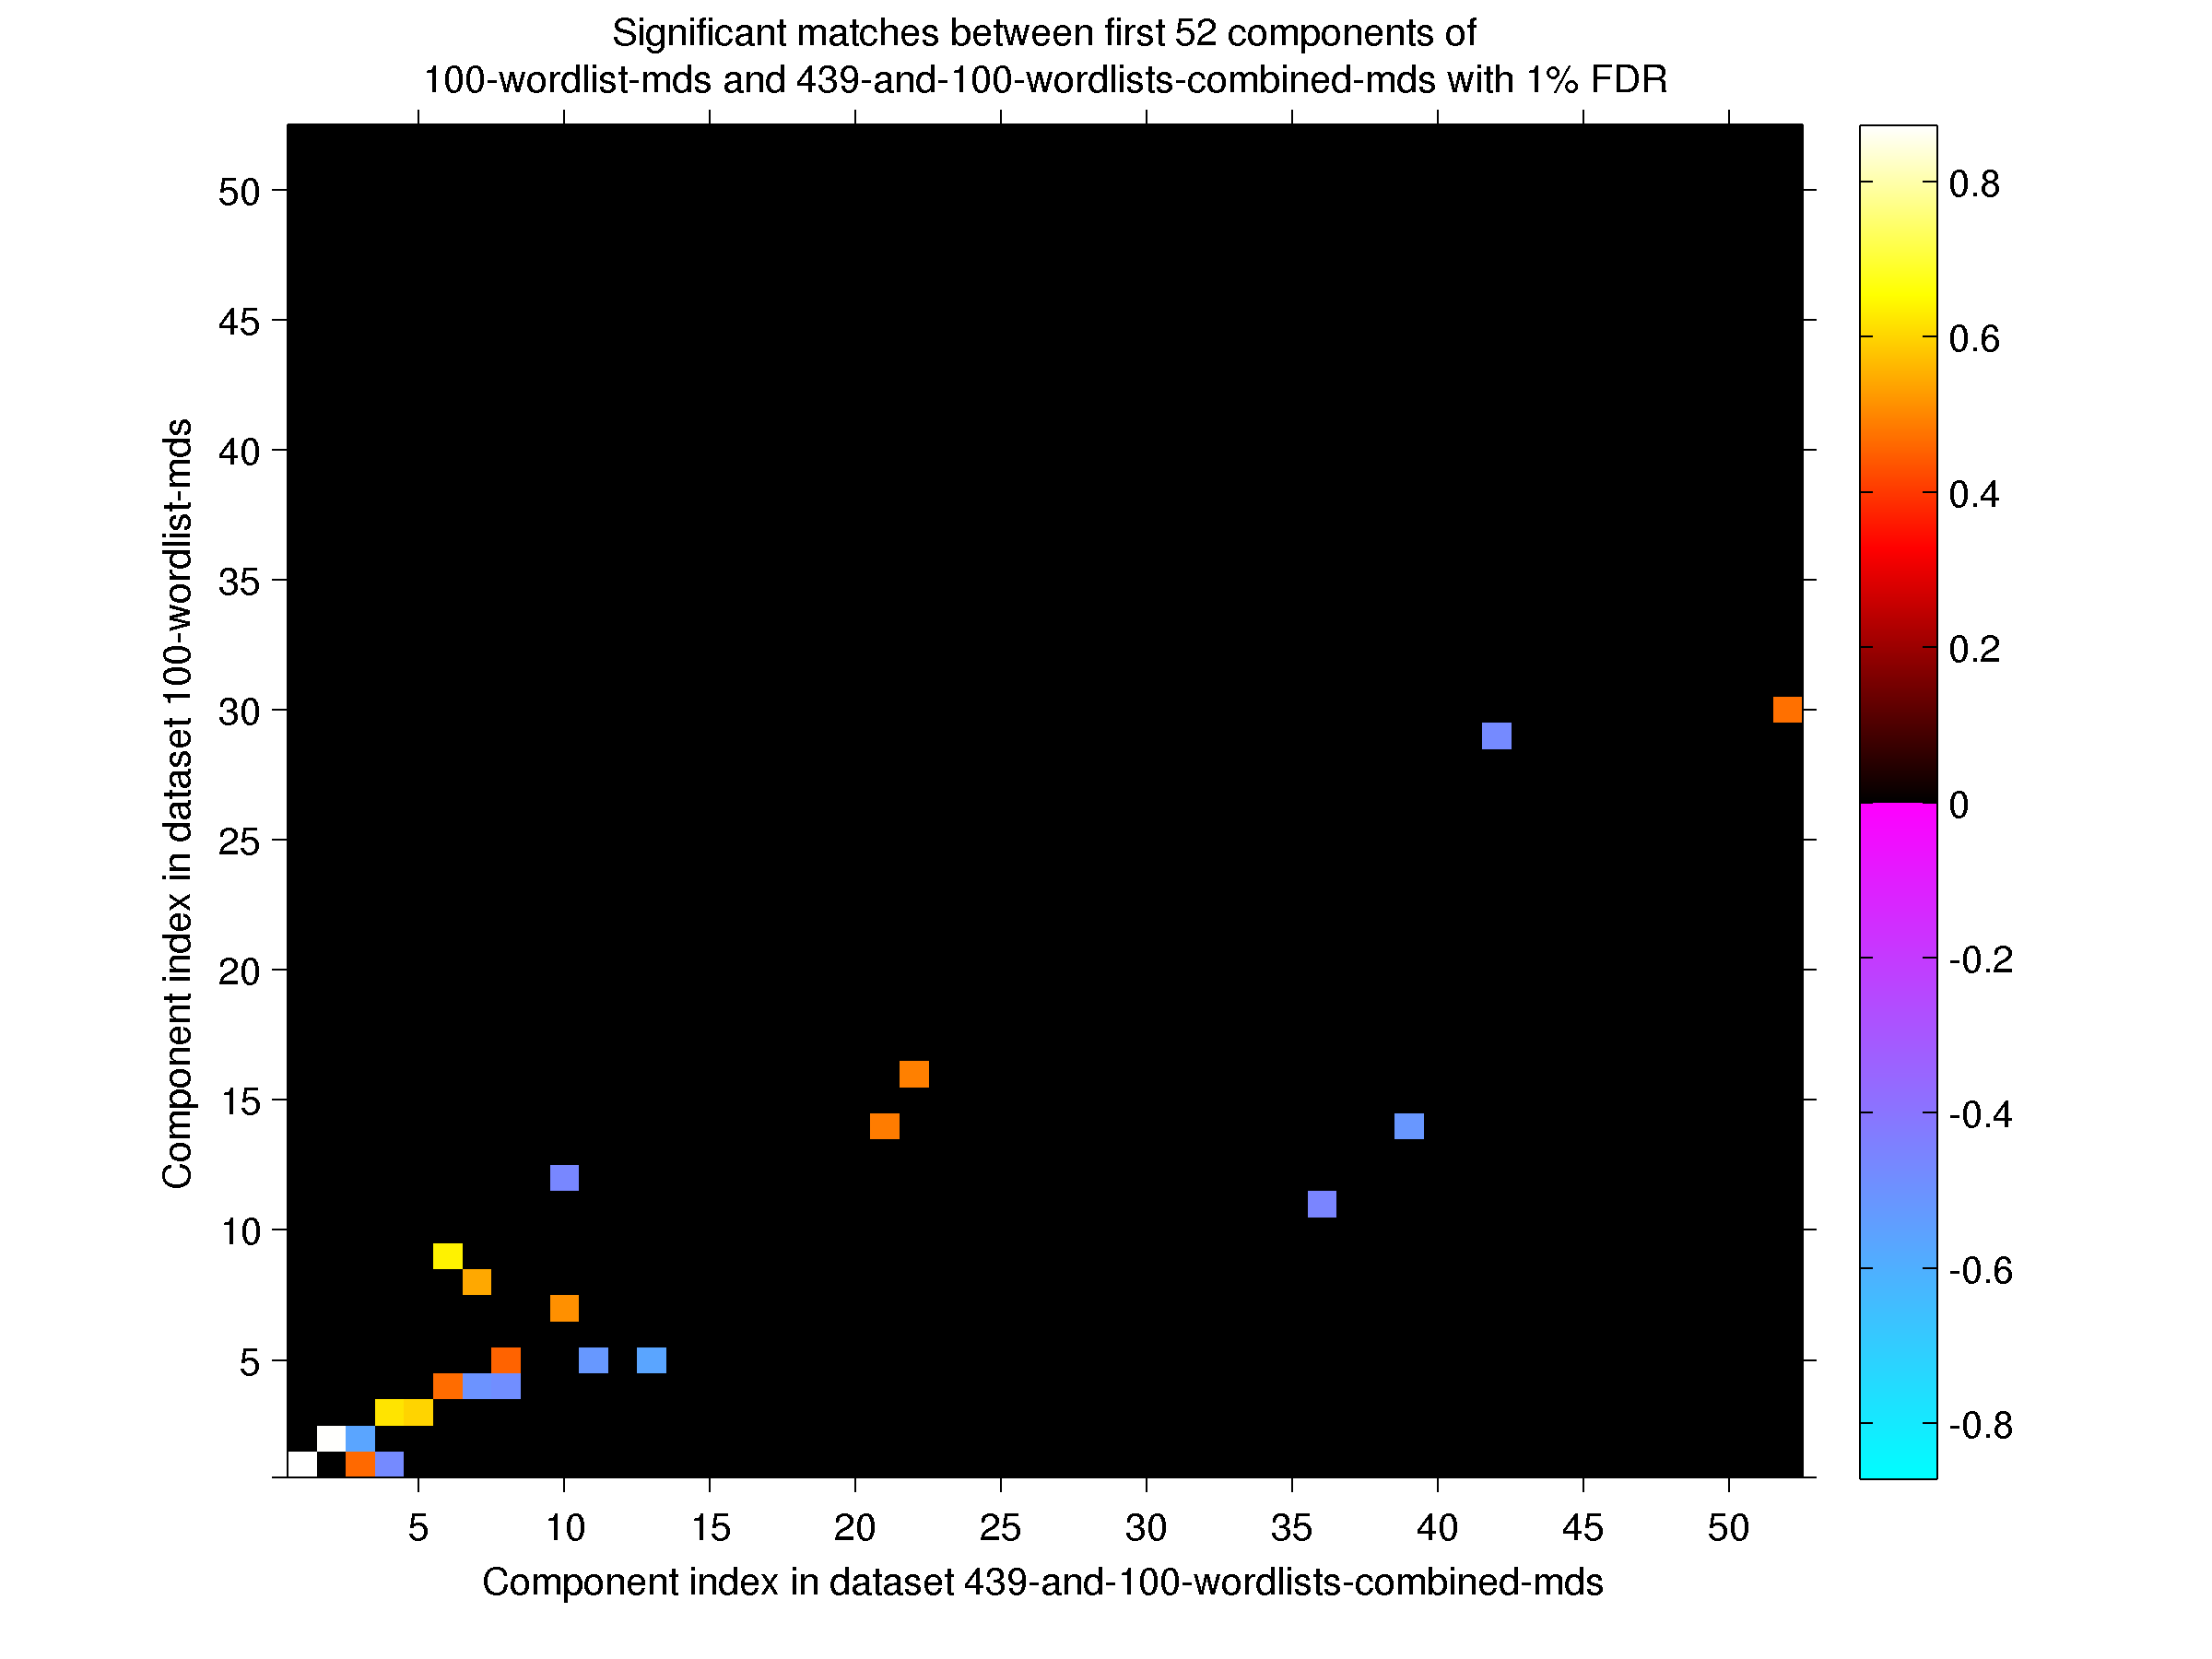
\includegraphics[width=0.9\linewidth]{100-vs-439and100-from-800dim-lowercase-wmt-model-significant-first-52}
    \caption{Results from Table 
    \ref{100-vs-439and100-from-800dim-lowercase-wmt-model-significant-first-52.tex} 
    displayed as an image. Colors (except black) give correlation for matching 
    dimensions.}
    \label{fig:100vs439And100First52}
\end{figure}

\subsection{First 22 dimensions of 100 vs 2797}

Finally, we look at only the matches between the first 22 dimensions of the
100 words and 2797 word datasets. Most of the components of the 2797 word list 
(with the exceptions of 2, 5, and 8 which have 2) have one match from the 100 
word list. This gives the 2797 word list 1.2 matches per component on average
vs. 1.7 for the 100 word list.
See Figure \ref{fig:100vs2797First22} and
Table 
\ref{100-vs-2797-from-800dim-lowercase-wmt-model-significant-first-22.tex}.


\begin{table}[!tbp]
    \begin{tabular}{| ll |}
        \hline
        \textbf{100-wordlist-mds dim} & \textbf{2797-wordlist-mds -- dim(correlation)}\\
        1 & 1(0.78), 2(0.48)\\
        2 & 2(-0.81)\\
        3 & 4(-0.69), 8(-0.55)\\
        4 & 3(0.47), 5(-0.52), 18(0.46), 21(-0.44)\\
        5 & 6(0.71), 12(-0.47), 17(0.49)\\
        6 & 7(-0.52)\\
        7 & 14(0.49)\\
        8 & 8(-0.48)\\
        9 & 5(-0.5)\\
        11 & 13(-0.6)\\
        \hline
    \end{tabular}
    \caption{Dimensions from dataset 100-wordlist-mds which had a significant correlation with a dimension from dataset 2797-wordlist-mds when only the first 22 dimensions were considered as potential matches for one another with FDR controlled at 1\%. Each entry gives the matching dimension and the correlation between them.}
    \label{100-vs-2797-from-800dim-lowercase-wmt-model-significant-first-22.tex}
\end{table}


\begin{figure}[!tbp]
    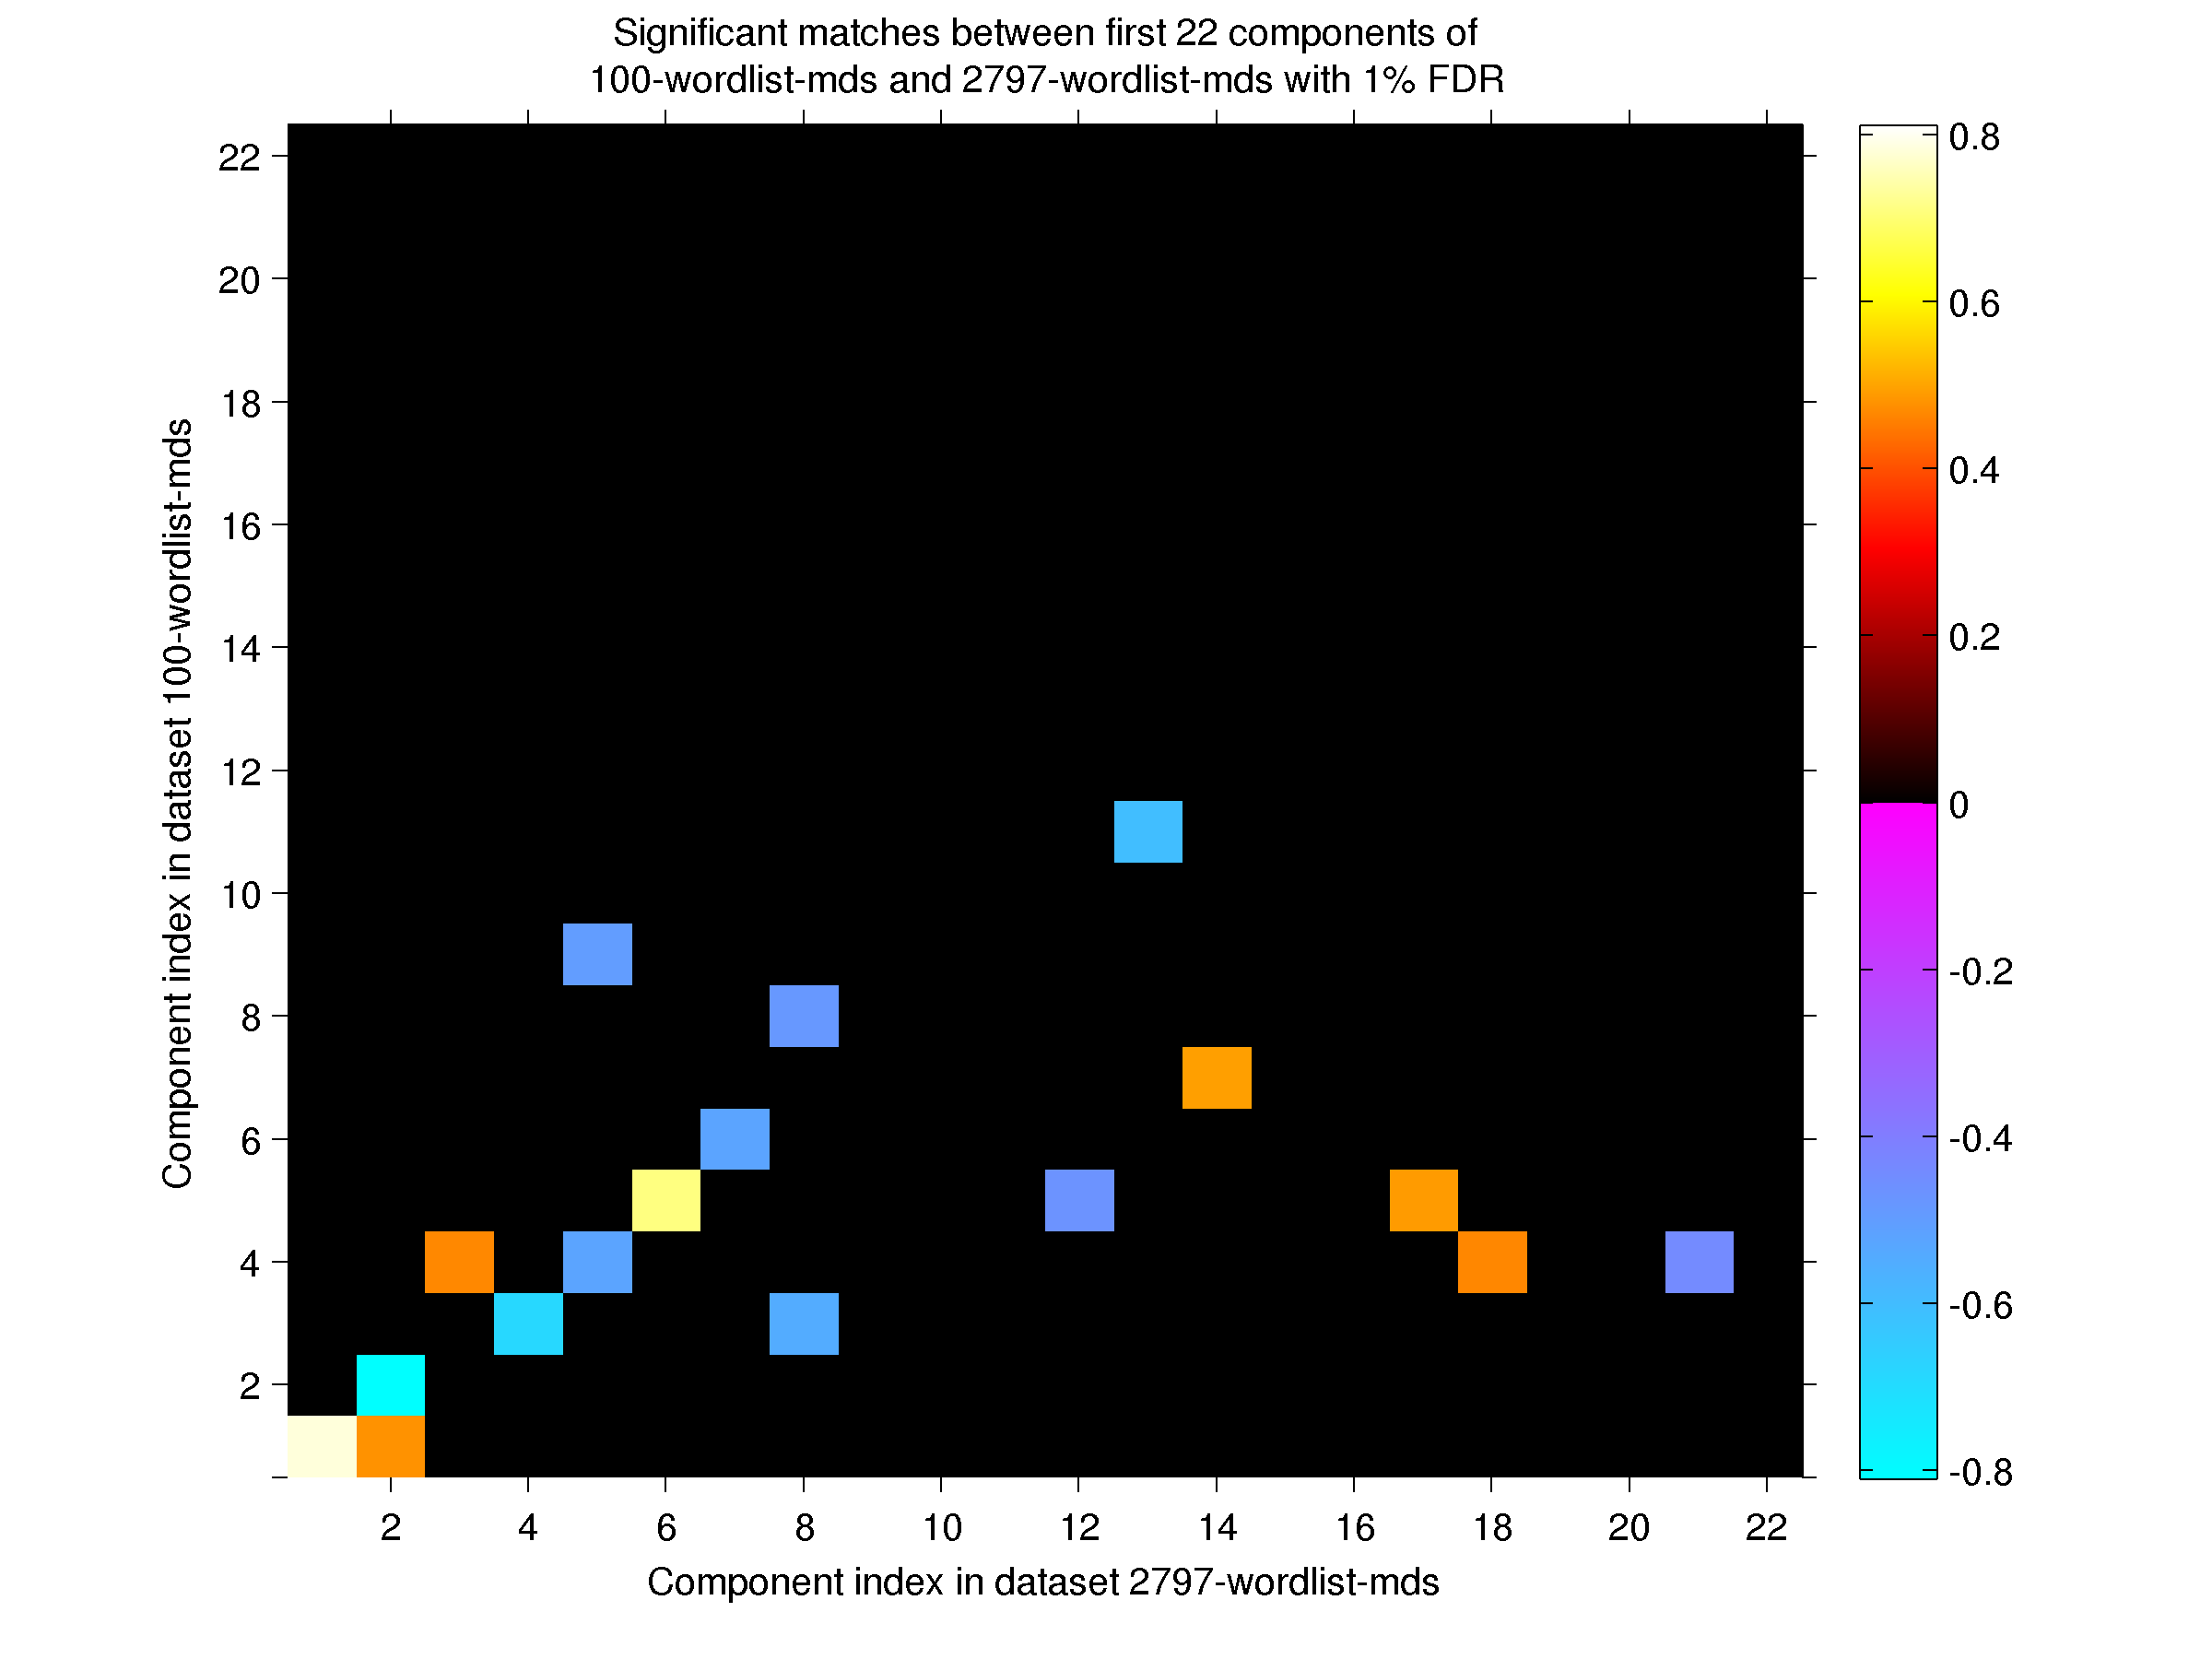
\includegraphics[width=0.9\linewidth]{100-vs-2797-from-800dim-lowercase-wmt-model-significant-first-22}
    \caption{Results from Table 
    \ref{100-vs-2797-from-800dim-lowercase-wmt-model-significant-first-22.tex} 
    displayed as an image. Colors (except black) give correlation for matching 
    dimensions.}
    \label{fig:100vs2797First22}
\end{figure}


\end{document}
